%%%%%%%%%%%%%%%%%%%
% Mathematics Department                 %
% FEU                                       %
% Undergraduate Thesis Template     %
% Edited May 2022                           %
%%%%%%%%%%%%%%%%%%%

\documentclass[12pt, a4paper]{report}
\usepackage{feumathstyle}  
\usepackage{amssymb, graphicx, amsmath}
\usepackage{hyperref}
\usepackage[T1]{fontenc}
\usepackage{apacite}
\bibliographystyle{apacite}

\usepackage{float}
\usepackage[english]{babel}


\usepackage{lscape}

\newtheorem{definition}{Definition}[chapter]
\newtheorem{theorem}{Theorem}[chapter]
\newtheorem{lemma}[theorem]{Lemma}
\newtheorem{corollary}[theorem]{Corollary}
\newtheorem{proposition}[theorem]{Proposition}

\begin{document}
	
	\title{Thesis Title} %do not capitalize all
	
	\authorfirst{Elisha Sophia S.}
	\authorlast{Borromeo}
	%\authorext{Jr.} 
	\authorexttrue %make this a comment if you do not have an extension name e.g. Jr., II, III, etc.

	\secondauthorfirst{Jan Edward F.}
	\secondauthorlast{Macagba}
	% \secondauthorext{Jr.} 
	\secondauthorexttrue %make this a comment if you do not have an extension name e.g. Jr., II, III, etc.

	\thirdauthorfirst{Consuelo B.}
	\thirdauthorlast{Mercado}
	%\thirdauthorext{Jr.} 
	\thirdauthorexttrue %make this a comment if you do not have an extension name e.g. Jr., II, III, etc.
	
	\degree{Bachelor of Science in Applied Mathematics } %enter the specific degree
	\thesistype{thesis} 
	\thesisdocument{undergraduate thesis} 
	
	\specialization{(Information Technology Track)} \specializetrue 
	
	\defensedate{May 12, 2022} %indicate the month, day and year the research was defended
	\submitmonth{May} %indicate the month the manuscript was submitted
	\submityear{2022} %indicate the year the manuscript was submitted 
	
	
	\adviser{May Anne C. Tirado, Ph.D.}%main adviser
	\panel{Panel, Ph.D.} 
	\secondpanel{Panel, Ph.D.} 
	\thirdpanel{Panel, Ph.D.} 
	

	\thesisinstructor{May Anne C. Tirado, Ph.D.} 
	
	
	%%%%%%%%%%%%%%%%%%%%%%%%%%%%%%%%%%%%%%%%%%%%%%%%%%%%%%%
	%% highlight \bothabsenttrue if the student has only one adviser and one reader
	%% otherwise comment \bothabsenttrue and highlight \coadviser or \coreader which 
	%% ever is applicable. In this case, the package assumes either you have 1 Adviser 
	%% and 2 Readers, or 2 Advisers and 1 Reader. 
	
	\bothabsenttrue
	
	%\coadviser{co-Adviser, Ph.D.} 
	%\coadvisetrue  
	% Make the \coadvisetrue as a comment if there is no adviser
	%%%%%%%%%%%%%%%%%%%%%%%%%%%%

	
	\deptchair{Genesis John G. Borja} 
	\dean{Rowena Capulong Reyes, Ph.D.}
	
	
	\abs{Type your abstract here.  Your abstract should have a minimum
		of 150 words and a maximum of 300 words.}
	
	\acknowledge{Type your acknowledgements here. It is customary to acknowledge special assistance from extramural agencies. There is no obligation that assistance received from members of the dissertation or thesis committee be acknowledged. \\
		Acknowledgments should be couched in terms consistent with the
		scholarly nature of the work. Your name and the date should not appear on this page.}
	
	
    	\beforepreface  
	\abstractpage
		
	\acknowledgetrue
	\acknowledgepage
	
	\tableofcontents
	
	\newpage


	\listoftables
	\listoffigures
	
	\afterpreface
	

	\chapter{The Problem and Its Background}

\label{chap:introduction}

\section{Background of the Study}

Flooding remains one of the major environmental challenges in the Philippines, particularly in highly urbanized areas where heavy rainfall, limited drainage capacity, and changes in land use contribute to the accumulation of surface water. In Metro Manila, flooding continues to affect residential communities, transportation systems, commercial establishments, and public infrastructure. Pasig City, which is situated near major waterways such as the Pasig River and is surrounded by densely developed urban areas, is among the locations that may experience flooding during periods of intense rainfall. These conditions highlight the importance of mathematical and computational approaches that can help predict flood behavior and improve the understanding of water movement in urban environments.
% TODO: add a citation for flooding in Metro Manila / Pasig City (e.g., a government or published source).

Flood prediction plays an important role in disaster risk reduction and urban planning. Accurate estimates of water depth and flow velocity can provide valuable information for identifying flood-prone areas and understanding the possible progression of inundation. Traditional hydrodynamic models simulate water movement by numerically solving governing mathematical equations. Although these models can be accurate, they are computationally slow and data-intensive \cite{liu2026}. \citeA{guo2021} noted that computational efficiency, model complexity, and the availability of high-quality input data are important challenges in urban flood modeling. The practical consequence of this cost was illustrated by \citeA{dikebreach2024}, who reported that simulating flood spread over a large area with a hydrodynamic model can take 6 to 10 hours, which is too long when authorities need predictions within seconds or minutes to support evacuation decisions.

Data-driven machine learning models offer a faster alternative. For example, the Long Short-Term Memory (LSTM) network of \citeA{dikebreach2024} produced flood-depth predictions in a fraction of a second after training. However, such models depend heavily on their training data, may behave as ``black boxes,'' and may produce predictions that violate physical principles \cite{liu2026,hybridreview2026}. In their systematic review of hybrid flood inundation models, \citeA{hybridreview2026} described this trade-off between the realism of physics-based models and the speed of machine learning models, and identified hybrid approaches as a way to combine the strengths of both.

The Shallow Water Equations (SWE) provide a mathematical representation of water movement by describing the conservation of mass and momentum in depth-averaged flow. These equations are widely used in flood modeling because they account for changes in water depth and horizontal velocity over space and time \cite{guo2021}. However, solving the SWE numerically may involve computational challenges, especially when dealing with complex terrain and spatially varying conditions.

Physics-Informed Neural Networks (PINNs) are one such hybrid approach. Introduced by \citeA{raissi2019}, PINNs incorporate governing differential equations into the loss function of a neural network, so that the network is trained to be consistent with both the available data and the governing physical laws. \citeA{hybridreview2026} identified PINNs as especially promising because they embed physical laws directly into machine learning. PINNs have since been applied to flood problems. \citeA{liu2026} developed a Shallow Water Equation-based PINN for urban flood depth prediction in Hongshan District, Wuhan, China, and reported better performance than DNN, CNN, and LSTM models. \citeA{tian2025} investigated PINNs for solving the two-dimensional SWE with terrain topography and rainfall source terms using benchmark cases. \citeA{praveen2024} developed a PINN for real-time flood prediction from rainfall-runoff data.

Despite these developments, important gaps remain. The framework of \citeA{liu2026} was developed for a single urban area and relied on simulated data, while the cases of \citeA{tian2025} were controlled benchmark problems rather than a specific real-world location. \citeA{praveen2024} used a publicly available dataset, so its real-world performance requires further validation. \citeA{hybridreview2026} also noted that hybrid flood models are evaluated using different datasets, conditions, and metrics, which makes them difficult to compare, and proposed standardized benchmarking against traditional hydrodynamic models. Consequently, the convergence, approximation error, and physical consistency of a SWE-based PINN in Pasig City have not been established.

In this study, a Shallow Water Equation-based Physics-Informed Neural Network will be developed and implemented in a selected area of Pasig City. The proposed model will be evaluated in terms of its convergence, approximation error, and ability to satisfy physical constraints. Its performance will also be compared with a classical numerical method to determine its effectiveness in solving the Shallow Water Equations for flood modeling.
\section{Statement of the Problem}

Flooding remains a significant concern in urban areas such as Pasig City, where rainfall, terrain elevation, and water flow conditions influence flood behavior. Predicting the movement and depth of floodwater requires a mathematical model that can represent the physical processes governing water flow. The Shallow Water Equations (SWE) provide such a representation, but solving them with classical numerical methods can be computationally demanding and dependent on detailed input data, particularly in complex urban settings \cite{guo2021,liu2026}. Meanwhile, purely data-driven approaches can be fast but depend heavily on their training data and may not satisfy the physical laws governing water movement \cite{liu2026,hybridreview2026}.

Physics-Informed Neural Networks (PINNs) combine neural network approximation with governing physical equations \cite{raissi2019}. Previous studies have applied PINNs to urban flood depth prediction \cite{liu2026}, to the two-dimensional SWE with terrain topography and rainfall source terms \cite{tian2025}, and to real-time flood prediction from rainfall-runoff data \cite{praveen2024}. However, these studies were conducted using their own study areas, datasets, and model configurations. They relied on simulated, benchmark, or publicly available data, and none of them applied a SWE-based PINN to Pasig City. Systematic comparisons of PINN convergence and approximation error against classical numerical methods across conditions also remain limited \cite{tian2025,hybridreview2026}. It therefore remains unestablished how a SWE-based PINN performs in Pasig City in terms of its convergence, approximation error, and ability to satisfy the conservation of mass and momentum.

The study will seek to answer the following general research question:

\begin{quote}
How can a Shallow Water Equation-based Physics-Informed Neural Network be developed and evaluated for predicting flood behavior in Pasig City?
\end{quote}

Specifically, the study will seek to answer the following questions:

\begin{enumerate}
    \item How can the Shallow Water Equations be formulated as the governing mathematical model for flood and water flow behavior in Pasig City?
    \item How can a Physics-Informed Neural Network be developed to incorporate the Shallow Water Equations into its training process?
    \item What are the convergence behavior and approximation error of the proposed PINN in solving the Shallow Water Equations?
    \item How does the performance of the PINN compare with that of a classical numerical method when evaluated using appropriate error metrics?
    \item To what extent does the proposed PINN satisfy the physical constraints of water flow, particularly the conservation of water mass and momentum?
\end{enumerate}

\section{General and Specific Objectives}

% Present the general and specific objectives of the study.

\subsection{General Objective}

The general objective of this study is to develop and evaluate a Shallow Water Equation-based Physics-Informed Neural Network for predicting flood behavior in Pasig City.

\subsection{Specific Objectives}

Specifically, this study aims to:

\begin{enumerate}
    \item Formulate the Shallow Water Equations as the governing mathematical model for flood and water flow behavior in Pasig City.

    \item Develop a Physics-Informed Neural Network that incorporates the Shallow Water Equations into its training process.

    \item Evaluate the convergence and approximation error of the proposed PINN in solving the Shallow Water Equations.

    \item Compare the performance of the PINN with a classical numerical method using appropriate error metrics.

    \item Assess the model's ability to satisfy physical constraints, particularly the conservation of water mass and momentum.
\end{enumerate}

%\section{Hypothesis}

% Present the hypotheses that will be tested in the study, particularly regarding the performance of the proposed SWE-based PINN compared with a classical numerical method.

%The following hypotheses will be tested to determine whether a significant difference exists between the convergence and approximation error of the proposed SWE-based Physics-Informed Neural Network and the classical numerical method.

%\begin{itemize}
    %\item \textbf{Null Hypothesis ($H_0$):} There is no significant difference between the convergence and approximation error of the SWE-based PINN and the classical numerical method in solving the Shallow Water Equations for flood modeling in Pasig City.

    %\item \textbf{Alternative Hypothesis ($H_1$):} There is a significant difference between the convergence and approximation error of the SWE-based PINN and the classical numerical method in solving the Shallow Water Equations for flood modeling in Pasig City.
%\end{itemize}

\section{Conceptual Framework}

% Present a conceptual framework illustrating the relationship between the input data, the SWE-based Physics-Informed Neural Network, and the predicted flood or water behavior.

% The framework should show how the input data, such as rainfall, terrain elevation, and initial and boundary conditions, are processed by the PINN. The Shallow Water Equations serve as physical constraints during model training, while the network produces predictions of water depth and velocity.

% The framework should illustrate the following components:

\begin{figure}[H]
    \centering
    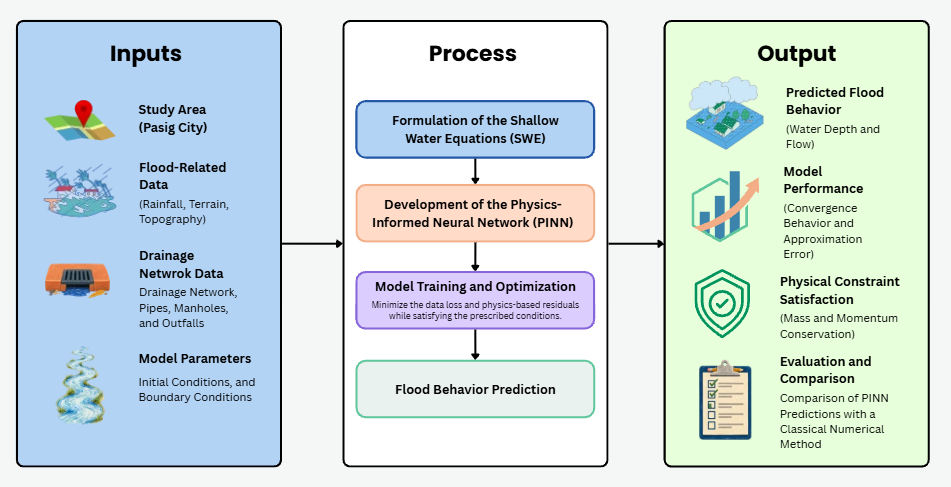
\includegraphics[width=0.95\textwidth]{assets/conceptual_framework.png}
    \caption{Conceptual Framework of the SWE-Based Physics-Informed Neural Network for Flood Modeling in Pasig City}
    \label{fig:conceptual_framework}
\end{figure}

The conceptual framework of the study follows an Input-Process-Output (IPO) model. It illustrates how the input data are processed through a Physics-Informed Neural Network incorporating the Shallow Water Equations to generate predictions of water depth, water flow, and flood behavior. 

\begin{enumerate}
    \item \textbf{Input Data:} The input data consist of rainfall data, terrain elevation, drainage network data, initial conditions, and boundary conditions for the selected study area in Pasig City. The drainage network data will provide information needed to incorporate the drainage rate into the governing equations. These inputs provide the environmental, spatial, and mathematical information required for the flood modeling process.

    \item \textbf{Process:} The input data will be processed using a SWE-based Physics-Informed Neural Network (PINN). The governing Shallow Water Equations, including the drainage rate as a representation of water removal through the drainage system, will be incorporated into the model's loss function as physical constraints. The network will undergo training and optimization by minimizing the data loss and the residuals of the governing equations while satisfying the specified initial and boundary conditions. Once trained, the model will be used to predict flood behavior across the selected study area.

    \item \textbf{Output:} The proposed model will generate predictions of water depth and horizontal water velocity, representing the flood behavior across the selected study area in Pasig City. The model will also be evaluated based on its convergence behavior, approximation error, and ability to satisfy the physical constraints represented by the conservation of mass and momentum.
\end{enumerate}

\section{Significance of the Study}

% Discuss the potential contributions of the study to flood modeling, disaster risk reduction, mathematical modeling, and the application of Physics-Informed Neural Networks. Identify the possible beneficiaries, such as local government units, disaster risk reduction offices, researchers, and future students.

This study aims to contribute to the development and evaluation of physics-informed computational approaches for flood modeling. By integrating the Shallow Water Equations into a neural network, the research will examine how physical constraints can be incorporated into flood prediction and how the resulting model performs compared with a classical numerical method.

\subsection{Local Government Units}

The findings of the study may provide useful information to local government units, particularly Pasig City, regarding the potential application of physics-informed neural networks in flood modeling. The predicted water depth and velocity may help improve the understanding of flood behavior in selected areas. However, the model is intended as a research-based computational approach and will not replace official flood forecasting systems.

\subsection{Disaster Risk Reduction and Management Offices}

The study may contribute to the development of computational approaches that can support flood assessment and disaster risk reduction. The results may provide additional insights into the movement and accumulation of water during flooding, which could be useful in understanding flood-prone areas.

\subsection{Researchers and the Academic Community}

This study may serve as a reference for researchers interested in mathematical modeling, numerical solutions of partial differential equations, and Physics-Informed Neural Networks. The comparison between the PINN and a classical numerical method may contribute to further investigations into the accuracy, convergence, and physical consistency of physics-informed models.

\subsection{Future Researchers and Students}

The study may serve as a foundation for future research involving PINNs and the Shallow Water Equations. Future researchers may extend the model by incorporating more detailed terrain data, additional hydrological variables, or more complex representations of urban drainage systems.

\section{Scope and Limitations}

% Define the coverage of the study, including the selected Philippine study area, the Shallow Water Equations, the input datasets, and the implementation of the SWE-based PINN.

% Discuss the limitations of the research, including data availability, spatial and temporal resolution, computational resources, and assumptions involved in the mathematical model.

This study will focus on the development and evaluation of a Shallow Water Equation-based Physics-Informed Neural Network for flood modeling in Pasig City, Philippines. The research will utilize the Shallow Water Equations as the governing mathematical model to represent the conservation of mass and momentum in water flow. The PINN will be developed to predict water depth and horizontal water velocity based on the available rainfall data, terrain elevation, initial conditions, and boundary conditions.

The study will evaluate the performance of the proposed PINN by comparing its numerical predictions with those obtained from a classical numerical method. The comparison will focus on convergence, approximation error, and physical consistency. Appropriate error metrics will be used to assess the differences between the two methods.

The scope of the study is limited to the selected study area within Pasig City and the available datasets. The accuracy of the model may be affected by the quality, completeness, and spatial and temporal resolution of the rainfall and terrain data. The availability of observed flood depth and water velocity measurements may also limit the extent of model validation.

Furthermore, the mathematical model will rely on the assumptions associated with the Shallow Water Equations, including the representation of water flow as a depth-averaged process. The study will not fully represent every physical factor that may influence urban flooding, such as highly detailed drainage network behavior, localized obstructions, or complex interactions between surface water and underground infrastructure. The model's computational performance may also depend on the available hardware and training configuration.

The study will primarily assess the PINN as a mathematical and computational approach to solving the Shallow Water Equations. Therefore, the findings will not necessarily establish the model's readiness for real-time operational flood forecasting or its applicability to all flood-prone areas in the Philippines.

\section{Definition of Terms}

% Provide the operational and conceptual definitions of important terms used throughout the study, including:

% Shallow Water Equations (SWE)
% Physics-Informed Neural Network (PINN)
% Flood Modeling
% Water Depth
% Horizontal Water Velocity
% Initial Conditions
% Boundary Conditions
% Approximation Error
% Convergence
% Conservation of Mass
% Conservation of Momentum

The following terms are defined conceptually and operationally to provide a clearer understanding of the concepts used in this study.

\begin{itemize}

    \item \textbf{Shallow Water Equations (SWE).}
    The Shallow Water Equations are a system of partial differential equations derived from the principles of conservation of mass and momentum. In this study, they serve as the governing mathematical model for representing water flow and flood behavior in Pasig City.

    \item \textbf{Physics-Informed Neural Network (PINN).}
    A Physics-Informed Neural Network is a neural network that incorporates governing physical equations into its training process through a loss function. In this study, the PINN will use the Shallow Water Equations as physical constraints to predict water depth and horizontal water velocity.

    \item \textbf{Flood Modeling.}
    Flood modeling refers to the mathematical and computational representation of flood behavior. In this study, it involves simulating water movement and estimating water depth and velocity within the selected study area.

    \item \textbf{Water Depth.}
    Water depth refers to the vertical distance between the ground surface and the water surface. In this study, it is one of the primary variables predicted by the SWE-based PINN.

    \item \textbf{Horizontal Water Velocity.}
    Horizontal water velocity refers to the rate and direction of water movement along the horizontal plane. In this study, it is represented by the velocity components in the $x$- and $y$-directions.

    \item \textbf{Initial Conditions.}
    Initial conditions specify the state of the modeled water system at the beginning of the simulation. In this study, they define the initial water depth and velocity values used in solving the Shallow Water Equations.

    \item \textbf{Boundary Conditions.}
    Boundary conditions describe the behavior of water flow along the boundaries of the computational domain. In this study, they define the constraints applied at the edges of the selected flood modeling area.

    \item \textbf{Approximation Error.}
    Approximation error refers to the difference between the solution produced by a computational method and a reference solution. In this study, it will be used to evaluate the accuracy of the PINN in comparison with the classical numerical method.

    \item \textbf{Convergence.}
    Convergence refers to the tendency of a numerical or computational solution to approach a stable or reference solution as the relevant approximation or training process progresses. In this study, it will be evaluated to examine the behavior of the PINN and the classical numerical method in solving the Shallow Water Equations.

    \item \textbf{Conservation of Mass.}
    Conservation of mass is the physical principle stating that mass is neither created nor destroyed within a system, although it may enter or leave through the system boundaries. In this study, it is represented by the continuity equation of the Shallow Water Equations.

    \item \textbf{Conservation of Momentum.}
    Conservation of momentum is the physical principle describing how the momentum of water changes due to forces such as gravity, friction, and flow interactions. In this study, it is represented by the momentum equations of the Shallow Water Equations.

\end{itemize}
	
\chapter{Review of Related Literature and Studies}

\label{chap:review}

This chapter presents the concepts, theories, literature, and previous studies relevant to the development of a Shallow Water Equation-based Physics-Informed Neural Network for flood prediction. Since the study combines several fields, namely mathematics, physics, machine learning, and flood prediction, the discussion is organized to establish the theoretical and scientific foundation of the proposed model.

\section{Preliminaries}

This section introduces the fundamental concepts necessary for understanding the study. It provides an overview of flooding, hydrodynamic modeling, artificial neural networks, and Physics-Informed Neural Networks.

\subsection{Fundamental Concepts of Flooding}

Discuss the basic concepts of flooding, including its causes, characteristics, and effects. Explain important flood-related variables such as water depth, flow velocity, rainfall, and surface runoff.

\subsection{Hydrodynamic Modeling}

Discuss hydrodynamic modeling and its role in simulating the movement and distribution of water. Introduce the use of mathematical equations and numerical methods in representing flood behavior.

\subsection{Artificial Neural Networks}

Introduce artificial neural networks, including their basic structure, components, and learning process. Explain how neural networks can be used to approximate complex mathematical relationships.

\subsection{Physics-Informed Neural Networks}

Discuss Physics-Informed Neural Networks and how physical laws and governing equations are incorporated into neural network training. Explain their advantages and limitations compared with purely data-driven approaches.

\section{Theoretical Background}

This section presents the mathematical and computational theories that serve as the foundation of the proposed SWE-based PINN.

\subsection{Shallow Water Equations}

Present the Shallow Water Equations and explain their application in modeling flood flow and water movement over terrain.

\subsection{Conservation of Mass}

Discuss the principle of conservation of mass and its mathematical representation in the Shallow Water Equations.

\subsection{Conservation of Momentum}

Explain the principle of conservation of momentum and its role in describing the movement and velocity of water.

\subsection{Governing Equations for Flood Flow}

Present the governing equations used to describe flood flow, including the relevant flux terms and source terms associated with terrain slope and friction.

\subsection{Physics-Informed Neural Network Framework}

Discuss the mathematical structure of the PINN, including its neural network architecture, input and output variables, automatic differentiation, and incorporation of the governing equations.

\subsection{Loss Function of a PINN}

Explain the components of the PINN loss function, including the data loss, initial and boundary condition losses, and physics-based residual loss. Discuss how these components guide the network toward physically consistent solutions.

\section{Review of Related Literature}

This section discusses existing literature, concepts, and theoretical discussions related to flood prediction, hydrodynamic modeling, and the application of machine learning and Physics-Informed Neural Networks.

\subsection{Flood Prediction and Modeling}

Review the existing approaches used in flood prediction and modeling, including traditional mathematical and computational techniques.

\subsection{Flood Modeling in Urban Areas}

Discuss the challenges of urban flood modeling, including complex terrain, land use, drainage systems, and surface runoff.

\subsection{Shallow Water Equation Applications}

Review the applications of the Shallow Water Equations in simulating water movement, flood propagation, and water depth distribution.

\subsection{Physics-Informed Neural Networks in Hydrology}

Discuss the use of PINNs in hydrological modeling, particularly their ability to incorporate physical constraints into data-driven prediction models.

\subsection{Machine Learning for Flood Prediction}

Review machine learning approaches used in flood prediction, including artificial neural networks and other data-driven methods. Discuss their strengths and limitations.

\subsection{Flood Risk in Pasig City and Metro Manila}

Discuss the flood-related conditions and challenges in Pasig City and Metro Manila. Include relevant information about rainfall, river systems, urban development, and flood susceptibility.

\section{Review of Related Studies}

This section presents previous research studies that are directly related to the proposed research. Focus on the methods, datasets, results, and findings of each study.

\subsection{SWE-Based Flood Prediction Studies}

Review previous studies that used the Shallow Water Equations for flood simulation and prediction. Discuss their numerical methods, model performance, and findings.

\subsection{PINN-Based Flood Prediction Studies}

Present research studies that implemented Physics-Informed Neural Networks for flood prediction. Discuss their model architectures, governing equations, training methods, and evaluation metrics.

\subsection{PINN Applications in Hydrodynamics}

Review studies that applied PINNs to hydrodynamic problems, particularly those involving fluid flow, water movement, and conservation laws.

\subsection{Flood Prediction Studies in the Philippines}

Present previous research conducted in the Philippines concerning flood prediction, flood modeling, and flood risk assessment. Discuss the methodologies and findings relevant to the selected study area.

\section{Synthesis of Literature}

Summarize the common findings, approaches, and limitations identified in the reviewed literature and studies. Discuss the similarities and differences between traditional hydrodynamic models, machine learning approaches, and Physics-Informed Neural Networks.

\section{Research Gap}

Identify the limitations and unresolved issues in previous research. Explain the need for further investigation into the convergence, approximation error, and physical consistency of SWE-based Physics-Informed Neural Networks for flood modeling.

\section{Relevance to the Present Study}

Explain how the reviewed literature and studies support the development of the proposed SWE-based PINN. Establish the connection between the existing research and the objectives of the present study, particularly its comparison with a classical numerical method.

\section{Chapter Summary}

Provide a summary of the important concepts, theories, literature, and studies discussed in this chapter. Highlight how these establish the foundation for the methodology and model development presented in the succeeding chapter.

	
\chapter{Research Methodology}

\label{chap:methodology}

This chapter presents the research methodology that will be followed in developing and evaluating the Shallow Water Equation-based Physics-Informed Neural Network (SWE-based PINN) for flood prediction in a selected study area in the Philippines. It discusses the research design, study location, data sources, model parameters, mathematical formulation, neural network architecture, data preprocessing, training procedure, validation methods, and data analysis procedures.

\section{Research Methodology}

This study will employ a computational and mathematical modeling approach to develop a Physics-Informed Neural Network based on the Shallow Water Equations. The proposed model will incorporate physical laws governing water flow into the neural network training process to predict water depth and horizontal water velocity.

The developed model will be evaluated by examining its convergence, approximation error, and consistency with the governing physical equations. Its performance will also be compared with a classical numerical method for solving the Shallow Water Equations.

\section{Research Design}

This study will utilize a quantitative, computational, and model-development research design. It will involve the mathematical formulation of the Shallow Water Equations, implementation of a Physics-Informed Neural Network, and numerical experiments to assess the model's performance.

The study will use quantitative evaluation metrics to measure prediction accuracy, convergence behavior, and physical consistency. Comparisons with a classical numerical method will be conducted to determine the performance of the proposed model.

\section{Research Locale and Period}

The study will focus on selected flood-prone areas in Pasig City, Philippines, particularly areas associated with the Pasig River and its relevant waterways.

The research will cover the period from [Start Date] to [End Date]. The selected study area and simulation domain will be determined based on the availability of geographical, rainfall, and hydrological datasets required for the mathematical model.

\section{Sources of Data}

The study will utilize secondary data obtained from relevant government agencies, public databases, and other reliable sources. These datasets will provide the necessary information for developing, training, and evaluating the proposed model.

The potential data requirements include:

\begin{itemize}
    \item \textbf{Rainfall Data:} Historical rainfall measurements from relevant meteorological monitoring stations.
    
    \item \textbf{Water-Level Data:} Historical water-level measurements from the Pasig River and other relevant waterways.
    
    \item \textbf{River Flow and Discharge Data:} Available measurements describing the movement and volume of water within the selected waterways.
    
    \item \textbf{Geographic and Elevation Data:} Digital Elevation Models (DEM) and other geographical information describing the terrain of the study area.
    
    \item \textbf{Historical Flood Observations:} Available records of flood occurrences, water depths, durations, and affected locations.
    
    \item \textbf{Initial and Boundary Conditions:} Data required to establish the initial state of the water system and the conditions along the boundaries of the simulation domain.
\end{itemize}

The final selection of datasets will depend on their availability, accessibility, completeness, and suitability for the proposed mathematical model.

\section{Model Parameters, Variables, and Initial/Boundary Conditions}

This section identifies the variables and parameters used in formulating and implementing the SWE-based PINN.

The model will consider the following variables:

\begin{itemize}
    \item \textbf{Spatial Coordinates:} The horizontal coordinates representing the position within the study area.
    
    \item \textbf{Time:} The temporal variable representing the progression of the flood simulation.
    
    \item \textbf{Water Depth:} The depth of water at a given spatial location and time.
    
    \item \textbf{Horizontal Water Velocity:} The velocity components describing water movement in the horizontal directions.
    
    \item \textbf{Rainfall:} Precipitation data that may contribute to the source terms of the governing equations.
\end{itemize}

The model parameters will include relevant physical quantities and numerical settings, such as gravitational acceleration, terrain elevation, friction coefficients, and other parameters required by the governing equations.

Initial and boundary conditions will be established using available hydrological and geographical information to define the behavior of the water system within the simulation domain.

\section{Mathematical Model Formulation}

This section presents the mathematical foundation of the proposed model using the Shallow Water Equations.

\subsection{Governing Shallow Water Equations}

Present the system of partial differential equations describing the movement of water across the selected study area.

\subsection{Conservation of Mass}

Discuss the continuity equation governing the conservation of water mass within the simulation domain.

\subsection{Conservation of Momentum}

Present the momentum equations describing changes in water velocity due to gravitational forces, terrain slope, and friction.

\subsection{Initial Conditions}

Define the initial water depth and horizontal velocity conditions at the beginning of the simulation.

\subsection{Boundary Conditions}

Specify the conditions imposed along the boundaries of the computational domain, including relevant inflow, outflow, or other boundary constraints.

\section{PINN Model Architecture}

This section describes the architecture and mathematical structure of the Physics-Informed Neural Network used to approximate the solutions of the Shallow Water Equations.

\subsection{Neural Network Structure}

Describe the neural network architecture, including its input layer, hidden layers, activation functions, and output layer.

\subsection{Input and Output Variables}

Identify the spatial coordinates and time as the primary network inputs. The outputs will represent the predicted water depth and horizontal water velocity components.

\subsection{Physics-Based Constraints}

Explain how the Shallow Water Equations are incorporated into the network using automatic differentiation to calculate the partial derivatives required for the governing equations.

\subsection{Loss Function Formulation}

Present the composite loss function, including the data loss, initial condition loss, boundary condition loss, and physics-based residual loss.

Explain how the different loss components are combined and minimized during training to obtain physically consistent predictions.

\section{Data Preprocessing}

This section discusses the procedures applied to the collected datasets before they are used in model development and training.

The preprocessing procedures may include:

\begin{itemize}
    \item Data cleaning and removal of invalid observations.
    \item Normalization or scaling of numerical variables.
    \item Identification and handling of missing data.
    \item Spatial and temporal alignment of datasets.
    \item Preparation of training, validation, and testing datasets.
\end{itemize}

These procedures will ensure that the collected data are suitable for numerical computation and neural network training.

\section{Model Training Procedure}

This section explains the process of training the SWE-based PINN.

The training procedure will involve defining the network architecture, initializing its parameters, calculating the composite loss function, and updating the network weights through an optimization algorithm.

The following aspects will be discussed:

\begin{itemize}
    \item Training and validation data preparation.
    \item Selection of optimization algorithms.
    \item Configuration of learning rates and training iterations.
    \item Selection of collocation points for evaluating the governing equations.
    \item Monitoring and minimization of the composite loss function.
    \item Evaluation of convergence during training.
\end{itemize}

\section{Model Validation and Evaluation}

The developed SWE-based PINN will be evaluated to determine its accuracy, convergence behavior, and physical consistency.

The evaluation will consider the following metrics:

\begin{itemize}
    \item \textbf{Root Mean Square Error (RMSE):} Measures the average magnitude of prediction errors while giving greater weight to larger errors.
    
    \item \textbf{Mean Absolute Error (MAE):} Measures the average absolute difference between predicted and reference values.
    
    \item \textbf{Coefficient of Determination ($R^2$):} Measures how well the model explains the variation in the reference data, where appropriate.
    
    \item \textbf{Physics-Based Residual Error:} Measures the extent to which the predicted solutions satisfy the governing Shallow Water Equations.
    
    \item \textbf{Convergence Analysis:} Examines the behavior of the model's loss function and approximation error throughout the training process.
\end{itemize}

The PINN predictions will be compared with available measured observations or numerical solutions obtained using a classical method for solving the Shallow Water Equations.

\section{Data Analysis Procedure}

The results generated by the proposed model will be analyzed using quantitative and numerical methods.

The analysis will focus on the following:

\begin{enumerate}
    \item Examining the convergence behavior of the PINN during training.
    
    \item Measuring the approximation error between the predicted and reference solutions.
    
    \item Evaluating the physical consistency of the predicted water depth and velocity using the governing equations.
    
    \item Comparing the performance of the PINN with a classical numerical method.
    
    \item Interpreting the results to determine the effectiveness and limitations of the proposed model for flood prediction.
\end{enumerate}

The findings will be presented using appropriate tables, graphs, and other visual representations to support the interpretation of the model's performance.

	\chapter{How to Cite References}
\label{chap:citing}

First edit the file {\tt bibliog.bib} by adding an entry for each
reference used in your thesis.  Follow the format in the sample
file.

\begin{verbatim}
@BOOK{bsw,
  author={H. T. Banks and R. C. Smith and Y. Wang},
  title={Smart Material Structures: Modeling Estimation
         and Control},
  year=1996,
  publisher={Masson/John Wiley},
  address={Paris/Chichester}
}

@ARTICLE{BanksIto1,
  author={H. T. Banks and K. Ito},
  year=1997,
  title={Approximation in {LQR} Problems for Infinite Dimensional
    Systems with Unbounded Input Operators},
  journal={Journal of Mathematical Systems, Estimation, and Control},
  volume=7,
  pages={1-34},
  publisher={Birkh\"{a}user Boston}
}

@PHDTHESIS{Ric,
  author = {R. C. H. del Rosario },
  year = 1998,
  title = {Computational Methods for Feedback Control in
        Structural Systems},
  school = {N. C. State University}
}

@techreport{RalphRic3a,
  author = {R. C. H. del Rosario and R. C. Smith},
  year = 1997,
  title = {{LQR} Control of Thin Shell Dynamics: Formulation and
           Numerical Implementation},
  institution = {Institute for Computer Applications in Science
    and Engineering},
  number={ICASE Report 97-59},
  address={NASA Langley Research Center, Hampton},
}

%%%%%%%%%%%%%%%%%%%%%%%%%%%%%   %MISC   %%%%%%%%%%%%%%%%%%%%%%%%%%%

@BOOKLET{Le,
  author={A. W. Leissa},
  title={Vibrations of Shells},
  year=1973,
  publisher={NASA SP-288},
  howpublished={Reprinted by the Acoustical Society of America 
  	through the American Institute of Physics}
}

@manual{d31ref,
  organization = {{Institute} of Electrical and 
  	Electronics Engineers},
  year = 1978,
  title = {IEEE Standard on Piezoelectricity},
  address={New York}
}

@manual{pside,
  title = {Specification of PSIDE},
  author={Jacques J.B. de Swart and Walter M. Lioen and 
  	Wolter A. van der Veen},
  year=1998,
  note={Avalable at http://www.cwi.nl/cwi/projects/PSIDE/}
}
\end{verbatim}


Click from the BibTex icon (if you are using WinEdit Program) or
use the BibTex command if you are in command line mode.  It is
suggested that you do this twice.  Then compile the main tex file
using the LaTeX command.

Use the {\tt cite} command to cite a reference.  For example,
\verb|\cite{bsw}| cites the book labeled
``bsw''. This will give us {\cite{bsw}}.

	%%%%% edit the chapter files. no more preamble. start directly on \chapter{}. add more as needed. you may rename the files and the code arguments accordingly
	
	\appendix
	
\chapter{ThesisMain.tex File}
\label{chap:Main}


The ThesisMain.tex file contains the basic information about your thesis while the chapter files are just called in the code.  This is the only file you need to compile. Do not run the chapter files.

\section{Preamble}

\begin{verbatim} 
	\documentclass[12pt]{report}
	\usepackage{feumathstyle}  
	\usepackage{amssymb, graphicx, amsmath}
	\usepackage{hyperref}
	\usepackage{apacite}
	\bibliographystyle{apacite}
	
	\usepackage{lscape}
	
	\newtheorem{definition}{Definition}[chapter]
	\newtheorem{theorem}{Theorem}[chapter]
	\newtheorem{lemma}[theorem]{Lemma}
	\newtheorem{corollary}[theorem]{Corollary}
	\newtheorem{proposition}[theorem]{Proposition}
 \end{verbatim}

you may add additional packages but do not remove the prelisted packages especially the feumathstyle package.
You may add other new formats here too


\section{Basic Information}

\begin{verbatim}
	\title{Thesis Title} %do not capitalize all

\authorfirst{Juan L.}
\authorlast{Dela Cruz}
\authorext{Jr.} 
\authorexttrue %make this a comment if you do not have an extension name e.g. Jr., II, III, etc.

\secondauthorfirst{Juan L.}
\secondauthorlast{Dela Cruz}
\secondauthorext{Jr.} 
\secondauthorexttrue %make this a comment if you do not have an extension name e.g. Jr., II, III, etc.

\thirdauthorfirst{Juan L.}
\thirdauthorlast{Dela Cruz}
\thirdauthorext{Jr.} 
\thirdauthorexttrue %make this a comment if you do not have an extension name e.g. Jr., II, III, etc.

\degree{Bachelor of Science in Applied Mathematics } %enter the specific degree
\thesistype{thesis} 
\thesisdocument{undergraduate thesis} 

\specialization{with Information Technology} \specializetrue 

\defensedate{May 12, 2022} %indicate the month, day and year the research was defended
\submitmonth{May} %indicate the month the manuscript was submitted
\submityear{2022} %indicate the year the manuscript was submitted 


\adviser{Adviser, Ph.D.}%main adviser
\panel{Panel, Ph.D.} 
\secondpanel{Panel, Ph.D.} 
\thirdpanel{Panel, Ph.D.} 


\thesisinstructor{May Anne C. Tirado, Ph.D.} 


%%%%%%%%%%%%%%%%%%%%%%%%%%%%%%%%%%%%%%%%%%%%%%%%%%%%%%%
%% highlight \bothabsenttrue if the student has only one adviser and one reader
%% otherwise comment \bothabsenttrue and highlight \coadviser or \coreader which 
%% ever is applicable. In this case, the package assumes either you have 1 Adviser 
%% and 2 Readers, or 2 Advisers and 1 Reader. 

\bothabsenttrue

%\coadviser{co-Adviser, Ph.D.} 
%\coadvisetrue  
% Make the \coadvisetrue as a comment if there is no adviser
%%%%%%%%%%%%%%%%%%%%%%%%%%%%


\deptchair{Genesis John G. Borja} 
\dean{Dean Name}
\end{verbatim}

input the names and information about your thesis, authors, adviser, panel, dean.

\section{Abstract and Acknowledgements}

\begin{verbatim}
		
	\abs{Type your abstract here.  Your abstract should have a minimum
		of 150 words and a maximum of 300 words.}
	
	\acknowledge{Type your acknowledgements here. It is customary to acknowledge special assistance from extramural agencies. There is no obligation that assistance received from members of the dissertation or thesis committee be acknowledged. \\
		Acknowledgments should be couched in terms consistent with the
		scholarly nature of the work. Your name and the date should not appear on this page.}
\end{verbatim}

type your abstract and acknowledgements here

\section{Chapters and Appendix}

Type your chapters and appendix in separate tex files. This is so it will be easier to edit a shorter code than the full manuscript. 

The chapter files starts with
\begin{verbatim}
	\chapter{How to Wrtie Text and Type Equations}
	\label{chap:typing}
\end{verbatim}	

The label is optional. This part is when you want to cite this chapter in other chapters. This file just ends with the last line of your chapter content.

\section{Document Outline}
\begin{verbatim} 
\beforepreface  
\abstractpage

\acknowledgetrue
\acknowledgepage

\tableofcontents

\newpage


\listoftables
\listoffigures

\afterpreface

\chapter{The Problem and Its Background}

\label{chap:introduction}

\section{Background of the Study}

Flooding remains one of the major environmental challenges in the Philippines, particularly in highly urbanized areas where heavy rainfall, limited drainage capacity, and changes in land use contribute to the accumulation of surface water. In Metro Manila, flooding continues to affect residential communities, transportation systems, commercial establishments, and public infrastructure. Pasig City, which is situated near major waterways such as the Pasig River and is surrounded by densely developed urban areas, is among the locations that may experience flooding during periods of intense rainfall. These conditions highlight the importance of mathematical and computational approaches that can help predict flood behavior and improve the understanding of water movement in urban environments.
% TODO: add a citation for flooding in Metro Manila / Pasig City (e.g., a government or published source).

Flood prediction plays an important role in disaster risk reduction and urban planning. Accurate estimates of water depth and flow velocity can provide valuable information for identifying flood-prone areas and understanding the possible progression of inundation. Traditional hydrodynamic models simulate water movement by numerically solving governing mathematical equations. Although these models can be accurate, they are computationally slow and data-intensive \cite{liu2026}. \citeA{guo2021} noted that computational efficiency, model complexity, and the availability of high-quality input data are important challenges in urban flood modeling. The practical consequence of this cost was illustrated by \citeA{dikebreach2024}, who reported that simulating flood spread over a large area with a hydrodynamic model can take 6 to 10 hours, which is too long when authorities need predictions within seconds or minutes to support evacuation decisions.

Data-driven machine learning models offer a faster alternative. For example, the Long Short-Term Memory (LSTM) network of \citeA{dikebreach2024} produced flood-depth predictions in a fraction of a second after training. However, such models depend heavily on their training data, may behave as ``black boxes,'' and may produce predictions that violate physical principles \cite{liu2026,hybridreview2026}. In their systematic review of hybrid flood inundation models, \citeA{hybridreview2026} described this trade-off between the realism of physics-based models and the speed of machine learning models, and identified hybrid approaches as a way to combine the strengths of both.

The Shallow Water Equations (SWE) provide a mathematical representation of water movement by describing the conservation of mass and momentum in depth-averaged flow. These equations are widely used in flood modeling because they account for changes in water depth and horizontal velocity over space and time \cite{guo2021}. However, solving the SWE numerically may involve computational challenges, especially when dealing with complex terrain and spatially varying conditions.

Physics-Informed Neural Networks (PINNs) are one such hybrid approach. Introduced by \citeA{raissi2019}, PINNs incorporate governing differential equations into the loss function of a neural network, so that the network is trained to be consistent with both the available data and the governing physical laws. \citeA{hybridreview2026} identified PINNs as especially promising because they embed physical laws directly into machine learning. PINNs have since been applied to flood problems. \citeA{liu2026} developed a Shallow Water Equation-based PINN for urban flood depth prediction in Hongshan District, Wuhan, China, and reported better performance than DNN, CNN, and LSTM models. \citeA{tian2025} investigated PINNs for solving the two-dimensional SWE with terrain topography and rainfall source terms using benchmark cases. \citeA{praveen2024} developed a PINN for real-time flood prediction from rainfall-runoff data.

Despite these developments, important gaps remain. The framework of \citeA{liu2026} was developed for a single urban area and relied on simulated data, while the cases of \citeA{tian2025} were controlled benchmark problems rather than a specific real-world location. \citeA{praveen2024} used a publicly available dataset, so its real-world performance requires further validation. \citeA{hybridreview2026} also noted that hybrid flood models are evaluated using different datasets, conditions, and metrics, which makes them difficult to compare, and proposed standardized benchmarking against traditional hydrodynamic models. Consequently, the convergence, approximation error, and physical consistency of a SWE-based PINN in Pasig City have not been established.

In this study, a Shallow Water Equation-based Physics-Informed Neural Network will be developed and implemented in a selected area of Pasig City. The proposed model will be evaluated in terms of its convergence, approximation error, and ability to satisfy physical constraints. Its performance will also be compared with a classical numerical method to determine its effectiveness in solving the Shallow Water Equations for flood modeling.
\section{Statement of the Problem}

Flooding remains a significant concern in urban areas such as Pasig City, where rainfall, terrain elevation, and water flow conditions influence flood behavior. Predicting the movement and depth of floodwater requires a mathematical model that can represent the physical processes governing water flow. The Shallow Water Equations (SWE) provide such a representation, but solving them with classical numerical methods can be computationally demanding and dependent on detailed input data, particularly in complex urban settings \cite{guo2021,liu2026}. Meanwhile, purely data-driven approaches can be fast but depend heavily on their training data and may not satisfy the physical laws governing water movement \cite{liu2026,hybridreview2026}.

Physics-Informed Neural Networks (PINNs) combine neural network approximation with governing physical equations \cite{raissi2019}. Previous studies have applied PINNs to urban flood depth prediction \cite{liu2026}, to the two-dimensional SWE with terrain topography and rainfall source terms \cite{tian2025}, and to real-time flood prediction from rainfall-runoff data \cite{praveen2024}. However, these studies were conducted using their own study areas, datasets, and model configurations. They relied on simulated, benchmark, or publicly available data, and none of them applied a SWE-based PINN to Pasig City. Systematic comparisons of PINN convergence and approximation error against classical numerical methods across conditions also remain limited \cite{tian2025,hybridreview2026}. It therefore remains unestablished how a SWE-based PINN performs in Pasig City in terms of its convergence, approximation error, and ability to satisfy the conservation of mass and momentum.

The study will seek to answer the following general research question:

\begin{quote}
How can a Shallow Water Equation-based Physics-Informed Neural Network be developed and evaluated for predicting flood behavior in Pasig City?
\end{quote}

Specifically, the study will seek to answer the following questions:

\begin{enumerate}
    \item How can the Shallow Water Equations be formulated as the governing mathematical model for flood and water flow behavior in Pasig City?
    \item How can a Physics-Informed Neural Network be developed to incorporate the Shallow Water Equations into its training process?
    \item What are the convergence behavior and approximation error of the proposed PINN in solving the Shallow Water Equations?
    \item How does the performance of the PINN compare with that of a classical numerical method when evaluated using appropriate error metrics?
    \item To what extent does the proposed PINN satisfy the physical constraints of water flow, particularly the conservation of water mass and momentum?
\end{enumerate}

\section{General and Specific Objectives}

% Present the general and specific objectives of the study.

\subsection{General Objective}

The general objective of this study is to develop and evaluate a Shallow Water Equation-based Physics-Informed Neural Network for predicting flood behavior in Pasig City.

\subsection{Specific Objectives}

Specifically, this study aims to:

\begin{enumerate}
    \item Formulate the Shallow Water Equations as the governing mathematical model for flood and water flow behavior in Pasig City.

    \item Develop a Physics-Informed Neural Network that incorporates the Shallow Water Equations into its training process.

    \item Evaluate the convergence and approximation error of the proposed PINN in solving the Shallow Water Equations.

    \item Compare the performance of the PINN with a classical numerical method using appropriate error metrics.

    \item Assess the model's ability to satisfy physical constraints, particularly the conservation of water mass and momentum.
\end{enumerate}

%\section{Hypothesis}

% Present the hypotheses that will be tested in the study, particularly regarding the performance of the proposed SWE-based PINN compared with a classical numerical method.

%The following hypotheses will be tested to determine whether a significant difference exists between the convergence and approximation error of the proposed SWE-based Physics-Informed Neural Network and the classical numerical method.

%\begin{itemize}
    %\item \textbf{Null Hypothesis ($H_0$):} There is no significant difference between the convergence and approximation error of the SWE-based PINN and the classical numerical method in solving the Shallow Water Equations for flood modeling in Pasig City.

    %\item \textbf{Alternative Hypothesis ($H_1$):} There is a significant difference between the convergence and approximation error of the SWE-based PINN and the classical numerical method in solving the Shallow Water Equations for flood modeling in Pasig City.
%\end{itemize}

\section{Conceptual Framework}

% Present a conceptual framework illustrating the relationship between the input data, the SWE-based Physics-Informed Neural Network, and the predicted flood or water behavior.

% The framework should show how the input data, such as rainfall, terrain elevation, and initial and boundary conditions, are processed by the PINN. The Shallow Water Equations serve as physical constraints during model training, while the network produces predictions of water depth and velocity.

% The framework should illustrate the following components:

\begin{figure}[H]
    \centering
    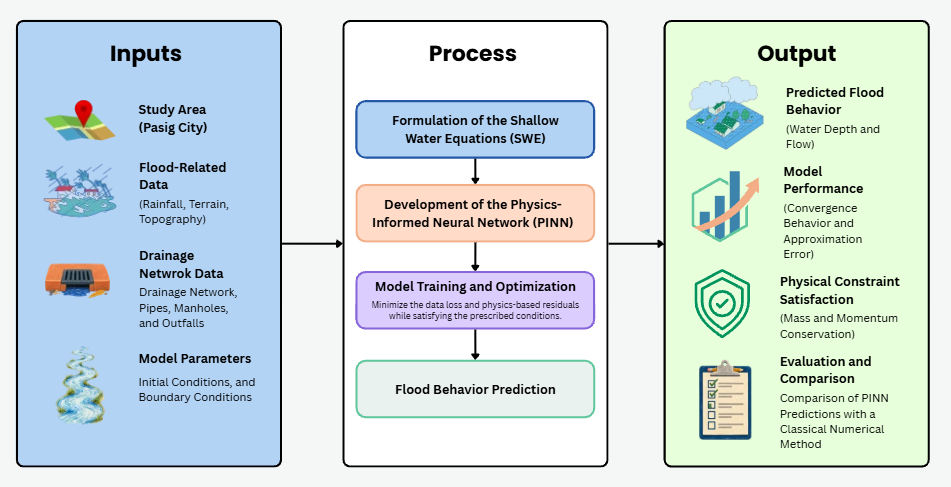
\includegraphics[width=0.95\textwidth]{assets/conceptual_framework.png}
    \caption{Conceptual Framework of the SWE-Based Physics-Informed Neural Network for Flood Modeling in Pasig City}
    \label{fig:conceptual_framework}
\end{figure}

The conceptual framework of the study follows an Input-Process-Output (IPO) model. It illustrates how the input data are processed through a Physics-Informed Neural Network incorporating the Shallow Water Equations to generate predictions of water depth, water flow, and flood behavior. 

\begin{enumerate}
    \item \textbf{Input Data:} The input data consist of rainfall data, terrain elevation, drainage network data, initial conditions, and boundary conditions for the selected study area in Pasig City. The drainage network data will provide information needed to incorporate the drainage rate into the governing equations. These inputs provide the environmental, spatial, and mathematical information required for the flood modeling process.

    \item \textbf{Process:} The input data will be processed using a SWE-based Physics-Informed Neural Network (PINN). The governing Shallow Water Equations, including the drainage rate as a representation of water removal through the drainage system, will be incorporated into the model's loss function as physical constraints. The network will undergo training and optimization by minimizing the data loss and the residuals of the governing equations while satisfying the specified initial and boundary conditions. Once trained, the model will be used to predict flood behavior across the selected study area.

    \item \textbf{Output:} The proposed model will generate predictions of water depth and horizontal water velocity, representing the flood behavior across the selected study area in Pasig City. The model will also be evaluated based on its convergence behavior, approximation error, and ability to satisfy the physical constraints represented by the conservation of mass and momentum.
\end{enumerate}

\section{Significance of the Study}

% Discuss the potential contributions of the study to flood modeling, disaster risk reduction, mathematical modeling, and the application of Physics-Informed Neural Networks. Identify the possible beneficiaries, such as local government units, disaster risk reduction offices, researchers, and future students.

This study aims to contribute to the development and evaluation of physics-informed computational approaches for flood modeling. By integrating the Shallow Water Equations into a neural network, the research will examine how physical constraints can be incorporated into flood prediction and how the resulting model performs compared with a classical numerical method.

\subsection{Local Government Units}

The findings of the study may provide useful information to local government units, particularly Pasig City, regarding the potential application of physics-informed neural networks in flood modeling. The predicted water depth and velocity may help improve the understanding of flood behavior in selected areas. However, the model is intended as a research-based computational approach and will not replace official flood forecasting systems.

\subsection{Disaster Risk Reduction and Management Offices}

The study may contribute to the development of computational approaches that can support flood assessment and disaster risk reduction. The results may provide additional insights into the movement and accumulation of water during flooding, which could be useful in understanding flood-prone areas.

\subsection{Researchers and the Academic Community}

This study may serve as a reference for researchers interested in mathematical modeling, numerical solutions of partial differential equations, and Physics-Informed Neural Networks. The comparison between the PINN and a classical numerical method may contribute to further investigations into the accuracy, convergence, and physical consistency of physics-informed models.

\subsection{Future Researchers and Students}

The study may serve as a foundation for future research involving PINNs and the Shallow Water Equations. Future researchers may extend the model by incorporating more detailed terrain data, additional hydrological variables, or more complex representations of urban drainage systems.

\section{Scope and Limitations}

% Define the coverage of the study, including the selected Philippine study area, the Shallow Water Equations, the input datasets, and the implementation of the SWE-based PINN.

% Discuss the limitations of the research, including data availability, spatial and temporal resolution, computational resources, and assumptions involved in the mathematical model.

This study will focus on the development and evaluation of a Shallow Water Equation-based Physics-Informed Neural Network for flood modeling in Pasig City, Philippines. The research will utilize the Shallow Water Equations as the governing mathematical model to represent the conservation of mass and momentum in water flow. The PINN will be developed to predict water depth and horizontal water velocity based on the available rainfall data, terrain elevation, initial conditions, and boundary conditions.

The study will evaluate the performance of the proposed PINN by comparing its numerical predictions with those obtained from a classical numerical method. The comparison will focus on convergence, approximation error, and physical consistency. Appropriate error metrics will be used to assess the differences between the two methods.

The scope of the study is limited to the selected study area within Pasig City and the available datasets. The accuracy of the model may be affected by the quality, completeness, and spatial and temporal resolution of the rainfall and terrain data. The availability of observed flood depth and water velocity measurements may also limit the extent of model validation.

Furthermore, the mathematical model will rely on the assumptions associated with the Shallow Water Equations, including the representation of water flow as a depth-averaged process. The study will not fully represent every physical factor that may influence urban flooding, such as highly detailed drainage network behavior, localized obstructions, or complex interactions between surface water and underground infrastructure. The model's computational performance may also depend on the available hardware and training configuration.

The study will primarily assess the PINN as a mathematical and computational approach to solving the Shallow Water Equations. Therefore, the findings will not necessarily establish the model's readiness for real-time operational flood forecasting or its applicability to all flood-prone areas in the Philippines.

\section{Definition of Terms}

% Provide the operational and conceptual definitions of important terms used throughout the study, including:

% Shallow Water Equations (SWE)
% Physics-Informed Neural Network (PINN)
% Flood Modeling
% Water Depth
% Horizontal Water Velocity
% Initial Conditions
% Boundary Conditions
% Approximation Error
% Convergence
% Conservation of Mass
% Conservation of Momentum

The following terms are defined conceptually and operationally to provide a clearer understanding of the concepts used in this study.

\begin{itemize}

    \item \textbf{Shallow Water Equations (SWE).}
    The Shallow Water Equations are a system of partial differential equations derived from the principles of conservation of mass and momentum. In this study, they serve as the governing mathematical model for representing water flow and flood behavior in Pasig City.

    \item \textbf{Physics-Informed Neural Network (PINN).}
    A Physics-Informed Neural Network is a neural network that incorporates governing physical equations into its training process through a loss function. In this study, the PINN will use the Shallow Water Equations as physical constraints to predict water depth and horizontal water velocity.

    \item \textbf{Flood Modeling.}
    Flood modeling refers to the mathematical and computational representation of flood behavior. In this study, it involves simulating water movement and estimating water depth and velocity within the selected study area.

    \item \textbf{Water Depth.}
    Water depth refers to the vertical distance between the ground surface and the water surface. In this study, it is one of the primary variables predicted by the SWE-based PINN.

    \item \textbf{Horizontal Water Velocity.}
    Horizontal water velocity refers to the rate and direction of water movement along the horizontal plane. In this study, it is represented by the velocity components in the $x$- and $y$-directions.

    \item \textbf{Initial Conditions.}
    Initial conditions specify the state of the modeled water system at the beginning of the simulation. In this study, they define the initial water depth and velocity values used in solving the Shallow Water Equations.

    \item \textbf{Boundary Conditions.}
    Boundary conditions describe the behavior of water flow along the boundaries of the computational domain. In this study, they define the constraints applied at the edges of the selected flood modeling area.

    \item \textbf{Approximation Error.}
    Approximation error refers to the difference between the solution produced by a computational method and a reference solution. In this study, it will be used to evaluate the accuracy of the PINN in comparison with the classical numerical method.

    \item \textbf{Convergence.}
    Convergence refers to the tendency of a numerical or computational solution to approach a stable or reference solution as the relevant approximation or training process progresses. In this study, it will be evaluated to examine the behavior of the PINN and the classical numerical method in solving the Shallow Water Equations.

    \item \textbf{Conservation of Mass.}
    Conservation of mass is the physical principle stating that mass is neither created nor destroyed within a system, although it may enter or leave through the system boundaries. In this study, it is represented by the continuity equation of the Shallow Water Equations.

    \item \textbf{Conservation of Momentum.}
    Conservation of momentum is the physical principle describing how the momentum of water changes due to forces such as gravity, friction, and flow interactions. In this study, it is represented by the momentum equations of the Shallow Water Equations.

\end{itemize}

\chapter{Review of Related Literature and Studies}

\label{chap:review}

This chapter presents the concepts, theories, literature, and previous studies relevant to the development of a Shallow Water Equation-based Physics-Informed Neural Network for flood prediction. Since the study combines several fields, namely mathematics, physics, machine learning, and flood prediction, the discussion is organized to establish the theoretical and scientific foundation of the proposed model.

\section{Preliminaries}

This section introduces the fundamental concepts necessary for understanding the study. It provides an overview of flooding, hydrodynamic modeling, artificial neural networks, and Physics-Informed Neural Networks.

\subsection{Fundamental Concepts of Flooding}

Discuss the basic concepts of flooding, including its causes, characteristics, and effects. Explain important flood-related variables such as water depth, flow velocity, rainfall, and surface runoff.

\subsection{Hydrodynamic Modeling}

Discuss hydrodynamic modeling and its role in simulating the movement and distribution of water. Introduce the use of mathematical equations and numerical methods in representing flood behavior.

\subsection{Artificial Neural Networks}

Introduce artificial neural networks, including their basic structure, components, and learning process. Explain how neural networks can be used to approximate complex mathematical relationships.

\subsection{Physics-Informed Neural Networks}

Discuss Physics-Informed Neural Networks and how physical laws and governing equations are incorporated into neural network training. Explain their advantages and limitations compared with purely data-driven approaches.

\section{Theoretical Background}

This section presents the mathematical and computational theories that serve as the foundation of the proposed SWE-based PINN.

\subsection{Shallow Water Equations}

Present the Shallow Water Equations and explain their application in modeling flood flow and water movement over terrain.

\subsection{Conservation of Mass}

Discuss the principle of conservation of mass and its mathematical representation in the Shallow Water Equations.

\subsection{Conservation of Momentum}

Explain the principle of conservation of momentum and its role in describing the movement and velocity of water.

\subsection{Governing Equations for Flood Flow}

Present the governing equations used to describe flood flow, including the relevant flux terms and source terms associated with terrain slope and friction.

\subsection{Physics-Informed Neural Network Framework}

Discuss the mathematical structure of the PINN, including its neural network architecture, input and output variables, automatic differentiation, and incorporation of the governing equations.

\subsection{Loss Function of a PINN}

Explain the components of the PINN loss function, including the data loss, initial and boundary condition losses, and physics-based residual loss. Discuss how these components guide the network toward physically consistent solutions.

\section{Review of Related Literature}

This section discusses existing literature, concepts, and theoretical discussions related to flood prediction, hydrodynamic modeling, and the application of machine learning and Physics-Informed Neural Networks.

\subsection{Flood Prediction and Modeling}

Review the existing approaches used in flood prediction and modeling, including traditional mathematical and computational techniques.

\subsection{Flood Modeling in Urban Areas}

Discuss the challenges of urban flood modeling, including complex terrain, land use, drainage systems, and surface runoff.

\subsection{Shallow Water Equation Applications}

Review the applications of the Shallow Water Equations in simulating water movement, flood propagation, and water depth distribution.

\subsection{Physics-Informed Neural Networks in Hydrology}

Discuss the use of PINNs in hydrological modeling, particularly their ability to incorporate physical constraints into data-driven prediction models.

\subsection{Machine Learning for Flood Prediction}

Review machine learning approaches used in flood prediction, including artificial neural networks and other data-driven methods. Discuss their strengths and limitations.

\subsection{Flood Risk in Pasig City and Metro Manila}

Discuss the flood-related conditions and challenges in Pasig City and Metro Manila. Include relevant information about rainfall, river systems, urban development, and flood susceptibility.

\section{Review of Related Studies}

This section presents previous research studies that are directly related to the proposed research. Focus on the methods, datasets, results, and findings of each study.

\subsection{SWE-Based Flood Prediction Studies}

Review previous studies that used the Shallow Water Equations for flood simulation and prediction. Discuss their numerical methods, model performance, and findings.

\subsection{PINN-Based Flood Prediction Studies}

Present research studies that implemented Physics-Informed Neural Networks for flood prediction. Discuss their model architectures, governing equations, training methods, and evaluation metrics.

\subsection{PINN Applications in Hydrodynamics}

Review studies that applied PINNs to hydrodynamic problems, particularly those involving fluid flow, water movement, and conservation laws.

\subsection{Flood Prediction Studies in the Philippines}

Present previous research conducted in the Philippines concerning flood prediction, flood modeling, and flood risk assessment. Discuss the methodologies and findings relevant to the selected study area.

\section{Synthesis of Literature}

Summarize the common findings, approaches, and limitations identified in the reviewed literature and studies. Discuss the similarities and differences between traditional hydrodynamic models, machine learning approaches, and Physics-Informed Neural Networks.

\section{Research Gap}

Identify the limitations and unresolved issues in previous research. Explain the need for further investigation into the convergence, approximation error, and physical consistency of SWE-based Physics-Informed Neural Networks for flood modeling.

\section{Relevance to the Present Study}

Explain how the reviewed literature and studies support the development of the proposed SWE-based PINN. Establish the connection between the existing research and the objectives of the present study, particularly its comparison with a classical numerical method.

\section{Chapter Summary}

Provide a summary of the important concepts, theories, literature, and studies discussed in this chapter. Highlight how these establish the foundation for the methodology and model development presented in the succeeding chapter.


\chapter{Research Methodology}

\label{chap:methodology}

This chapter presents the research methodology that will be followed in developing and evaluating the Shallow Water Equation-based Physics-Informed Neural Network (SWE-based PINN) for flood prediction in a selected study area in the Philippines. It discusses the research design, study location, data sources, model parameters, mathematical formulation, neural network architecture, data preprocessing, training procedure, validation methods, and data analysis procedures.

\section{Research Methodology}

This study will employ a computational and mathematical modeling approach to develop a Physics-Informed Neural Network based on the Shallow Water Equations. The proposed model will incorporate physical laws governing water flow into the neural network training process to predict water depth and horizontal water velocity.

The developed model will be evaluated by examining its convergence, approximation error, and consistency with the governing physical equations. Its performance will also be compared with a classical numerical method for solving the Shallow Water Equations.

\section{Research Design}

This study will utilize a quantitative, computational, and model-development research design. It will involve the mathematical formulation of the Shallow Water Equations, implementation of a Physics-Informed Neural Network, and numerical experiments to assess the model's performance.

The study will use quantitative evaluation metrics to measure prediction accuracy, convergence behavior, and physical consistency. Comparisons with a classical numerical method will be conducted to determine the performance of the proposed model.

\section{Research Locale and Period}

The study will focus on selected flood-prone areas in Pasig City, Philippines, particularly areas associated with the Pasig River and its relevant waterways.

The research will cover the period from [Start Date] to [End Date]. The selected study area and simulation domain will be determined based on the availability of geographical, rainfall, and hydrological datasets required for the mathematical model.

\section{Sources of Data}

The study will utilize secondary data obtained from relevant government agencies, public databases, and other reliable sources. These datasets will provide the necessary information for developing, training, and evaluating the proposed model.

The potential data requirements include:

\begin{itemize}
    \item \textbf{Rainfall Data:} Historical rainfall measurements from relevant meteorological monitoring stations.
    
    \item \textbf{Water-Level Data:} Historical water-level measurements from the Pasig River and other relevant waterways.
    
    \item \textbf{River Flow and Discharge Data:} Available measurements describing the movement and volume of water within the selected waterways.
    
    \item \textbf{Geographic and Elevation Data:} Digital Elevation Models (DEM) and other geographical information describing the terrain of the study area.
    
    \item \textbf{Historical Flood Observations:} Available records of flood occurrences, water depths, durations, and affected locations.
    
    \item \textbf{Initial and Boundary Conditions:} Data required to establish the initial state of the water system and the conditions along the boundaries of the simulation domain.
\end{itemize}

The final selection of datasets will depend on their availability, accessibility, completeness, and suitability for the proposed mathematical model.

\section{Model Parameters, Variables, and Initial/Boundary Conditions}

This section identifies the variables and parameters used in formulating and implementing the SWE-based PINN.

The model will consider the following variables:

\begin{itemize}
    \item \textbf{Spatial Coordinates:} The horizontal coordinates representing the position within the study area.
    
    \item \textbf{Time:} The temporal variable representing the progression of the flood simulation.
    
    \item \textbf{Water Depth:} The depth of water at a given spatial location and time.
    
    \item \textbf{Horizontal Water Velocity:} The velocity components describing water movement in the horizontal directions.
    
    \item \textbf{Rainfall:} Precipitation data that may contribute to the source terms of the governing equations.
\end{itemize}

The model parameters will include relevant physical quantities and numerical settings, such as gravitational acceleration, terrain elevation, friction coefficients, and other parameters required by the governing equations.

Initial and boundary conditions will be established using available hydrological and geographical information to define the behavior of the water system within the simulation domain.

\section{Mathematical Model Formulation}

This section presents the mathematical foundation of the proposed model using the Shallow Water Equations.

\subsection{Governing Shallow Water Equations}

Present the system of partial differential equations describing the movement of water across the selected study area.

\subsection{Conservation of Mass}

Discuss the continuity equation governing the conservation of water mass within the simulation domain.

\subsection{Conservation of Momentum}

Present the momentum equations describing changes in water velocity due to gravitational forces, terrain slope, and friction.

\subsection{Initial Conditions}

Define the initial water depth and horizontal velocity conditions at the beginning of the simulation.

\subsection{Boundary Conditions}

Specify the conditions imposed along the boundaries of the computational domain, including relevant inflow, outflow, or other boundary constraints.

\section{PINN Model Architecture}

This section describes the architecture and mathematical structure of the Physics-Informed Neural Network used to approximate the solutions of the Shallow Water Equations.

\subsection{Neural Network Structure}

Describe the neural network architecture, including its input layer, hidden layers, activation functions, and output layer.

\subsection{Input and Output Variables}

Identify the spatial coordinates and time as the primary network inputs. The outputs will represent the predicted water depth and horizontal water velocity components.

\subsection{Physics-Based Constraints}

Explain how the Shallow Water Equations are incorporated into the network using automatic differentiation to calculate the partial derivatives required for the governing equations.

\subsection{Loss Function Formulation}

Present the composite loss function, including the data loss, initial condition loss, boundary condition loss, and physics-based residual loss.

Explain how the different loss components are combined and minimized during training to obtain physically consistent predictions.

\section{Data Preprocessing}

This section discusses the procedures applied to the collected datasets before they are used in model development and training.

The preprocessing procedures may include:

\begin{itemize}
    \item Data cleaning and removal of invalid observations.
    \item Normalization or scaling of numerical variables.
    \item Identification and handling of missing data.
    \item Spatial and temporal alignment of datasets.
    \item Preparation of training, validation, and testing datasets.
\end{itemize}

These procedures will ensure that the collected data are suitable for numerical computation and neural network training.

\section{Model Training Procedure}

This section explains the process of training the SWE-based PINN.

The training procedure will involve defining the network architecture, initializing its parameters, calculating the composite loss function, and updating the network weights through an optimization algorithm.

The following aspects will be discussed:

\begin{itemize}
    \item Training and validation data preparation.
    \item Selection of optimization algorithms.
    \item Configuration of learning rates and training iterations.
    \item Selection of collocation points for evaluating the governing equations.
    \item Monitoring and minimization of the composite loss function.
    \item Evaluation of convergence during training.
\end{itemize}

\section{Model Validation and Evaluation}

The developed SWE-based PINN will be evaluated to determine its accuracy, convergence behavior, and physical consistency.

The evaluation will consider the following metrics:

\begin{itemize}
    \item \textbf{Root Mean Square Error (RMSE):} Measures the average magnitude of prediction errors while giving greater weight to larger errors.
    
    \item \textbf{Mean Absolute Error (MAE):} Measures the average absolute difference between predicted and reference values.
    
    \item \textbf{Coefficient of Determination ($R^2$):} Measures how well the model explains the variation in the reference data, where appropriate.
    
    \item \textbf{Physics-Based Residual Error:} Measures the extent to which the predicted solutions satisfy the governing Shallow Water Equations.
    
    \item \textbf{Convergence Analysis:} Examines the behavior of the model's loss function and approximation error throughout the training process.
\end{itemize}

The PINN predictions will be compared with available measured observations or numerical solutions obtained using a classical method for solving the Shallow Water Equations.

\section{Data Analysis Procedure}

The results generated by the proposed model will be analyzed using quantitative and numerical methods.

The analysis will focus on the following:

\begin{enumerate}
    \item Examining the convergence behavior of the PINN during training.
    
    \item Measuring the approximation error between the predicted and reference solutions.
    
    \item Evaluating the physical consistency of the predicted water depth and velocity using the governing equations.
    
    \item Comparing the performance of the PINN with a classical numerical method.
    
    \item Interpreting the results to determine the effectiveness and limitations of the proposed model for flood prediction.
\end{enumerate}

The findings will be presented using appropriate tables, graphs, and other visual representations to support the interpretation of the model's performance.

\chapter{How to Cite References}
\label{chap:citing}

First edit the file {\tt bibliog.bib} by adding an entry for each
reference used in your thesis.  Follow the format in the sample
file.

\begin{verbatim}
@BOOK{bsw,
  author={H. T. Banks and R. C. Smith and Y. Wang},
  title={Smart Material Structures: Modeling Estimation
         and Control},
  year=1996,
  publisher={Masson/John Wiley},
  address={Paris/Chichester}
}

@ARTICLE{BanksIto1,
  author={H. T. Banks and K. Ito},
  year=1997,
  title={Approximation in {LQR} Problems for Infinite Dimensional
    Systems with Unbounded Input Operators},
  journal={Journal of Mathematical Systems, Estimation, and Control},
  volume=7,
  pages={1-34},
  publisher={Birkh\"{a}user Boston}
}

@PHDTHESIS{Ric,
  author = {R. C. H. del Rosario },
  year = 1998,
  title = {Computational Methods for Feedback Control in
        Structural Systems},
  school = {N. C. State University}
}

@techreport{RalphRic3a,
  author = {R. C. H. del Rosario and R. C. Smith},
  year = 1997,
  title = {{LQR} Control of Thin Shell Dynamics: Formulation and
           Numerical Implementation},
  institution = {Institute for Computer Applications in Science
    and Engineering},
  number={ICASE Report 97-59},
  address={NASA Langley Research Center, Hampton},
}

%%%%%%%%%%%%%%%%%%%%%%%%%%%%%   %MISC   %%%%%%%%%%%%%%%%%%%%%%%%%%%

@BOOKLET{Le,
  author={A. W. Leissa},
  title={Vibrations of Shells},
  year=1973,
  publisher={NASA SP-288},
  howpublished={Reprinted by the Acoustical Society of America 
  	through the American Institute of Physics}
}

@manual{d31ref,
  organization = {{Institute} of Electrical and 
  	Electronics Engineers},
  year = 1978,
  title = {IEEE Standard on Piezoelectricity},
  address={New York}
}

@manual{pside,
  title = {Specification of PSIDE},
  author={Jacques J.B. de Swart and Walter M. Lioen and 
  	Wolter A. van der Veen},
  year=1998,
  note={Avalable at http://www.cwi.nl/cwi/projects/PSIDE/}
}
\end{verbatim}


Click from the BibTex icon (if you are using WinEdit Program) or
use the BibTex command if you are in command line mode.  It is
suggested that you do this twice.  Then compile the main tex file
using the LaTeX command.

Use the {\tt cite} command to cite a reference.  For example,
\verb|\cite{bsw}| cites the book labeled
``bsw''. This will give us {\cite{bsw}}.

%%%%% edit the chapter files. no more preamble. start directly on \chapter{}. add more as needed. you may rename the files and the code arguments accordingly

\appendix

\chapter{ThesisMain.tex File}
\label{chap:Main}


The ThesisMain.tex file contains the basic information about your thesis while the chapter files are just called in the code.  This is the only file you need to compile. Do not run the chapter files.

\section{Preamble}

\begin{verbatim} 
	\documentclass[12pt]{report}
	\usepackage{feumathstyle}  
	\usepackage{amssymb, graphicx, amsmath}
	\usepackage{hyperref}
	\usepackage{apacite}
	\bibliographystyle{apacite}
	
	\usepackage{lscape}
	
	\newtheorem{definition}{Definition}[chapter]
	\newtheorem{theorem}{Theorem}[chapter]
	\newtheorem{lemma}[theorem]{Lemma}
	\newtheorem{corollary}[theorem]{Corollary}
	\newtheorem{proposition}[theorem]{Proposition}
 \end{verbatim}

you may add additional packages but do not remove the prelisted packages especially the feumathstyle package.
You may add other new formats here too


\section{Basic Information}

\begin{verbatim}
	\title{Thesis Title} %do not capitalize all

\authorfirst{Juan L.}
\authorlast{Dela Cruz}
\authorext{Jr.} 
\authorexttrue %make this a comment if you do not have an extension name e.g. Jr., II, III, etc.

\secondauthorfirst{Juan L.}
\secondauthorlast{Dela Cruz}
\secondauthorext{Jr.} 
\secondauthorexttrue %make this a comment if you do not have an extension name e.g. Jr., II, III, etc.

\thirdauthorfirst{Juan L.}
\thirdauthorlast{Dela Cruz}
\thirdauthorext{Jr.} 
\thirdauthorexttrue %make this a comment if you do not have an extension name e.g. Jr., II, III, etc.

\degree{Bachelor of Science in Applied Mathematics } %enter the specific degree
\thesistype{thesis} 
\thesisdocument{undergraduate thesis} 

\specialization{with Information Technology} \specializetrue 

\defensedate{May 12, 2022} %indicate the month, day and year the research was defended
\submitmonth{May} %indicate the month the manuscript was submitted
\submityear{2022} %indicate the year the manuscript was submitted 


\adviser{Adviser, Ph.D.}%main adviser
\panel{Panel, Ph.D.} 
\secondpanel{Panel, Ph.D.} 
\thirdpanel{Panel, Ph.D.} 


\thesisinstructor{May Anne C. Tirado, Ph.D.} 


%%%%%%%%%%%%%%%%%%%%%%%%%%%%%%%%%%%%%%%%%%%%%%%%%%%%%%%
%% highlight \bothabsenttrue if the student has only one adviser and one reader
%% otherwise comment \bothabsenttrue and highlight \coadviser or \coreader which 
%% ever is applicable. In this case, the package assumes either you have 1 Adviser 
%% and 2 Readers, or 2 Advisers and 1 Reader. 

\bothabsenttrue

%\coadviser{co-Adviser, Ph.D.} 
%\coadvisetrue  
% Make the \coadvisetrue as a comment if there is no adviser
%%%%%%%%%%%%%%%%%%%%%%%%%%%%


\deptchair{Genesis John G. Borja} 
\dean{Dean Name}
\end{verbatim}

input the names and information about your thesis, authors, adviser, panel, dean.

\section{Abstract and Acknowledgements}

\begin{verbatim}
		
	\abs{Type your abstract here.  Your abstract should have a minimum
		of 150 words and a maximum of 300 words.}
	
	\acknowledge{Type your acknowledgements here. It is customary to acknowledge special assistance from extramural agencies. There is no obligation that assistance received from members of the dissertation or thesis committee be acknowledged. \\
		Acknowledgments should be couched in terms consistent with the
		scholarly nature of the work. Your name and the date should not appear on this page.}
\end{verbatim}

type your abstract and acknowledgements here

\section{Chapters and Appendix}

Type your chapters and appendix in separate tex files. This is so it will be easier to edit a shorter code than the full manuscript. 

The chapter files starts with
\begin{verbatim}
	\chapter{How to Wrtie Text and Type Equations}
	\label{chap:typing}
\end{verbatim}	

The label is optional. This part is when you want to cite this chapter in other chapters. This file just ends with the last line of your chapter content.

\section{Document Outline}
\begin{verbatim} 
\beforepreface  
\abstractpage

\acknowledgetrue
\acknowledgepage

\tableofcontents

\newpage


\listoftables
\listoffigures

\afterpreface

\chapter{The Problem and Its Background}

\label{chap:introduction}

\section{Background of the Study}

Flooding remains one of the major environmental challenges in the Philippines, particularly in highly urbanized areas where heavy rainfall, limited drainage capacity, and changes in land use contribute to the accumulation of surface water. In Metro Manila, flooding continues to affect residential communities, transportation systems, commercial establishments, and public infrastructure. Pasig City, which is situated near major waterways such as the Pasig River and is surrounded by densely developed urban areas, is among the locations that may experience flooding during periods of intense rainfall. These conditions highlight the importance of mathematical and computational approaches that can help predict flood behavior and improve the understanding of water movement in urban environments.
% TODO: add a citation for flooding in Metro Manila / Pasig City (e.g., a government or published source).

Flood prediction plays an important role in disaster risk reduction and urban planning. Accurate estimates of water depth and flow velocity can provide valuable information for identifying flood-prone areas and understanding the possible progression of inundation. Traditional hydrodynamic models simulate water movement by numerically solving governing mathematical equations. Although these models can be accurate, they are computationally slow and data-intensive \cite{liu2026}. \citeA{guo2021} noted that computational efficiency, model complexity, and the availability of high-quality input data are important challenges in urban flood modeling. The practical consequence of this cost was illustrated by \citeA{dikebreach2024}, who reported that simulating flood spread over a large area with a hydrodynamic model can take 6 to 10 hours, which is too long when authorities need predictions within seconds or minutes to support evacuation decisions.

Data-driven machine learning models offer a faster alternative. For example, the Long Short-Term Memory (LSTM) network of \citeA{dikebreach2024} produced flood-depth predictions in a fraction of a second after training. However, such models depend heavily on their training data, may behave as ``black boxes,'' and may produce predictions that violate physical principles \cite{liu2026,hybridreview2026}. In their systematic review of hybrid flood inundation models, \citeA{hybridreview2026} described this trade-off between the realism of physics-based models and the speed of machine learning models, and identified hybrid approaches as a way to combine the strengths of both.

The Shallow Water Equations (SWE) provide a mathematical representation of water movement by describing the conservation of mass and momentum in depth-averaged flow. These equations are widely used in flood modeling because they account for changes in water depth and horizontal velocity over space and time \cite{guo2021}. However, solving the SWE numerically may involve computational challenges, especially when dealing with complex terrain and spatially varying conditions.

Physics-Informed Neural Networks (PINNs) are one such hybrid approach. Introduced by \citeA{raissi2019}, PINNs incorporate governing differential equations into the loss function of a neural network, so that the network is trained to be consistent with both the available data and the governing physical laws. \citeA{hybridreview2026} identified PINNs as especially promising because they embed physical laws directly into machine learning. PINNs have since been applied to flood problems. \citeA{liu2026} developed a Shallow Water Equation-based PINN for urban flood depth prediction in Hongshan District, Wuhan, China, and reported better performance than DNN, CNN, and LSTM models. \citeA{tian2025} investigated PINNs for solving the two-dimensional SWE with terrain topography and rainfall source terms using benchmark cases. \citeA{praveen2024} developed a PINN for real-time flood prediction from rainfall-runoff data.

Despite these developments, important gaps remain. The framework of \citeA{liu2026} was developed for a single urban area and relied on simulated data, while the cases of \citeA{tian2025} were controlled benchmark problems rather than a specific real-world location. \citeA{praveen2024} used a publicly available dataset, so its real-world performance requires further validation. \citeA{hybridreview2026} also noted that hybrid flood models are evaluated using different datasets, conditions, and metrics, which makes them difficult to compare, and proposed standardized benchmarking against traditional hydrodynamic models. Consequently, the convergence, approximation error, and physical consistency of a SWE-based PINN in Pasig City have not been established.

In this study, a Shallow Water Equation-based Physics-Informed Neural Network will be developed and implemented in a selected area of Pasig City. The proposed model will be evaluated in terms of its convergence, approximation error, and ability to satisfy physical constraints. Its performance will also be compared with a classical numerical method to determine its effectiveness in solving the Shallow Water Equations for flood modeling.
\section{Statement of the Problem}

Flooding remains a significant concern in urban areas such as Pasig City, where rainfall, terrain elevation, and water flow conditions influence flood behavior. Predicting the movement and depth of floodwater requires a mathematical model that can represent the physical processes governing water flow. The Shallow Water Equations (SWE) provide such a representation, but solving them with classical numerical methods can be computationally demanding and dependent on detailed input data, particularly in complex urban settings \cite{guo2021,liu2026}. Meanwhile, purely data-driven approaches can be fast but depend heavily on their training data and may not satisfy the physical laws governing water movement \cite{liu2026,hybridreview2026}.

Physics-Informed Neural Networks (PINNs) combine neural network approximation with governing physical equations \cite{raissi2019}. Previous studies have applied PINNs to urban flood depth prediction \cite{liu2026}, to the two-dimensional SWE with terrain topography and rainfall source terms \cite{tian2025}, and to real-time flood prediction from rainfall-runoff data \cite{praveen2024}. However, these studies were conducted using their own study areas, datasets, and model configurations. They relied on simulated, benchmark, or publicly available data, and none of them applied a SWE-based PINN to Pasig City. Systematic comparisons of PINN convergence and approximation error against classical numerical methods across conditions also remain limited \cite{tian2025,hybridreview2026}. It therefore remains unestablished how a SWE-based PINN performs in Pasig City in terms of its convergence, approximation error, and ability to satisfy the conservation of mass and momentum.

The study will seek to answer the following general research question:

\begin{quote}
How can a Shallow Water Equation-based Physics-Informed Neural Network be developed and evaluated for predicting flood behavior in Pasig City?
\end{quote}

Specifically, the study will seek to answer the following questions:

\begin{enumerate}
    \item How can the Shallow Water Equations be formulated as the governing mathematical model for flood and water flow behavior in Pasig City?
    \item How can a Physics-Informed Neural Network be developed to incorporate the Shallow Water Equations into its training process?
    \item What are the convergence behavior and approximation error of the proposed PINN in solving the Shallow Water Equations?
    \item How does the performance of the PINN compare with that of a classical numerical method when evaluated using appropriate error metrics?
    \item To what extent does the proposed PINN satisfy the physical constraints of water flow, particularly the conservation of water mass and momentum?
\end{enumerate}

\section{General and Specific Objectives}

% Present the general and specific objectives of the study.

\subsection{General Objective}

The general objective of this study is to develop and evaluate a Shallow Water Equation-based Physics-Informed Neural Network for predicting flood behavior in Pasig City.

\subsection{Specific Objectives}

Specifically, this study aims to:

\begin{enumerate}
    \item Formulate the Shallow Water Equations as the governing mathematical model for flood and water flow behavior in Pasig City.

    \item Develop a Physics-Informed Neural Network that incorporates the Shallow Water Equations into its training process.

    \item Evaluate the convergence and approximation error of the proposed PINN in solving the Shallow Water Equations.

    \item Compare the performance of the PINN with a classical numerical method using appropriate error metrics.

    \item Assess the model's ability to satisfy physical constraints, particularly the conservation of water mass and momentum.
\end{enumerate}

%\section{Hypothesis}

% Present the hypotheses that will be tested in the study, particularly regarding the performance of the proposed SWE-based PINN compared with a classical numerical method.

%The following hypotheses will be tested to determine whether a significant difference exists between the convergence and approximation error of the proposed SWE-based Physics-Informed Neural Network and the classical numerical method.

%\begin{itemize}
    %\item \textbf{Null Hypothesis ($H_0$):} There is no significant difference between the convergence and approximation error of the SWE-based PINN and the classical numerical method in solving the Shallow Water Equations for flood modeling in Pasig City.

    %\item \textbf{Alternative Hypothesis ($H_1$):} There is a significant difference between the convergence and approximation error of the SWE-based PINN and the classical numerical method in solving the Shallow Water Equations for flood modeling in Pasig City.
%\end{itemize}

\section{Conceptual Framework}

% Present a conceptual framework illustrating the relationship between the input data, the SWE-based Physics-Informed Neural Network, and the predicted flood or water behavior.

% The framework should show how the input data, such as rainfall, terrain elevation, and initial and boundary conditions, are processed by the PINN. The Shallow Water Equations serve as physical constraints during model training, while the network produces predictions of water depth and velocity.

% The framework should illustrate the following components:

\begin{figure}[H]
    \centering
    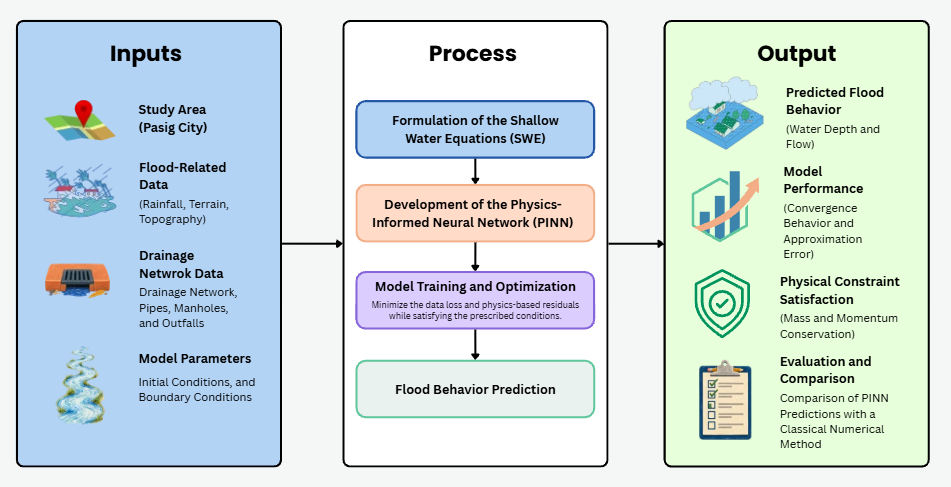
\includegraphics[width=0.95\textwidth]{assets/conceptual_framework.png}
    \caption{Conceptual Framework of the SWE-Based Physics-Informed Neural Network for Flood Modeling in Pasig City}
    \label{fig:conceptual_framework}
\end{figure}

The conceptual framework of the study follows an Input-Process-Output (IPO) model. It illustrates how the input data are processed through a Physics-Informed Neural Network incorporating the Shallow Water Equations to generate predictions of water depth, water flow, and flood behavior. 

\begin{enumerate}
    \item \textbf{Input Data:} The input data consist of rainfall data, terrain elevation, drainage network data, initial conditions, and boundary conditions for the selected study area in Pasig City. The drainage network data will provide information needed to incorporate the drainage rate into the governing equations. These inputs provide the environmental, spatial, and mathematical information required for the flood modeling process.

    \item \textbf{Process:} The input data will be processed using a SWE-based Physics-Informed Neural Network (PINN). The governing Shallow Water Equations, including the drainage rate as a representation of water removal through the drainage system, will be incorporated into the model's loss function as physical constraints. The network will undergo training and optimization by minimizing the data loss and the residuals of the governing equations while satisfying the specified initial and boundary conditions. Once trained, the model will be used to predict flood behavior across the selected study area.

    \item \textbf{Output:} The proposed model will generate predictions of water depth and horizontal water velocity, representing the flood behavior across the selected study area in Pasig City. The model will also be evaluated based on its convergence behavior, approximation error, and ability to satisfy the physical constraints represented by the conservation of mass and momentum.
\end{enumerate}

\section{Significance of the Study}

% Discuss the potential contributions of the study to flood modeling, disaster risk reduction, mathematical modeling, and the application of Physics-Informed Neural Networks. Identify the possible beneficiaries, such as local government units, disaster risk reduction offices, researchers, and future students.

This study aims to contribute to the development and evaluation of physics-informed computational approaches for flood modeling. By integrating the Shallow Water Equations into a neural network, the research will examine how physical constraints can be incorporated into flood prediction and how the resulting model performs compared with a classical numerical method.

\subsection{Local Government Units}

The findings of the study may provide useful information to local government units, particularly Pasig City, regarding the potential application of physics-informed neural networks in flood modeling. The predicted water depth and velocity may help improve the understanding of flood behavior in selected areas. However, the model is intended as a research-based computational approach and will not replace official flood forecasting systems.

\subsection{Disaster Risk Reduction and Management Offices}

The study may contribute to the development of computational approaches that can support flood assessment and disaster risk reduction. The results may provide additional insights into the movement and accumulation of water during flooding, which could be useful in understanding flood-prone areas.

\subsection{Researchers and the Academic Community}

This study may serve as a reference for researchers interested in mathematical modeling, numerical solutions of partial differential equations, and Physics-Informed Neural Networks. The comparison between the PINN and a classical numerical method may contribute to further investigations into the accuracy, convergence, and physical consistency of physics-informed models.

\subsection{Future Researchers and Students}

The study may serve as a foundation for future research involving PINNs and the Shallow Water Equations. Future researchers may extend the model by incorporating more detailed terrain data, additional hydrological variables, or more complex representations of urban drainage systems.

\section{Scope and Limitations}

% Define the coverage of the study, including the selected Philippine study area, the Shallow Water Equations, the input datasets, and the implementation of the SWE-based PINN.

% Discuss the limitations of the research, including data availability, spatial and temporal resolution, computational resources, and assumptions involved in the mathematical model.

This study will focus on the development and evaluation of a Shallow Water Equation-based Physics-Informed Neural Network for flood modeling in Pasig City, Philippines. The research will utilize the Shallow Water Equations as the governing mathematical model to represent the conservation of mass and momentum in water flow. The PINN will be developed to predict water depth and horizontal water velocity based on the available rainfall data, terrain elevation, initial conditions, and boundary conditions.

The study will evaluate the performance of the proposed PINN by comparing its numerical predictions with those obtained from a classical numerical method. The comparison will focus on convergence, approximation error, and physical consistency. Appropriate error metrics will be used to assess the differences between the two methods.

The scope of the study is limited to the selected study area within Pasig City and the available datasets. The accuracy of the model may be affected by the quality, completeness, and spatial and temporal resolution of the rainfall and terrain data. The availability of observed flood depth and water velocity measurements may also limit the extent of model validation.

Furthermore, the mathematical model will rely on the assumptions associated with the Shallow Water Equations, including the representation of water flow as a depth-averaged process. The study will not fully represent every physical factor that may influence urban flooding, such as highly detailed drainage network behavior, localized obstructions, or complex interactions between surface water and underground infrastructure. The model's computational performance may also depend on the available hardware and training configuration.

The study will primarily assess the PINN as a mathematical and computational approach to solving the Shallow Water Equations. Therefore, the findings will not necessarily establish the model's readiness for real-time operational flood forecasting or its applicability to all flood-prone areas in the Philippines.

\section{Definition of Terms}

% Provide the operational and conceptual definitions of important terms used throughout the study, including:

% Shallow Water Equations (SWE)
% Physics-Informed Neural Network (PINN)
% Flood Modeling
% Water Depth
% Horizontal Water Velocity
% Initial Conditions
% Boundary Conditions
% Approximation Error
% Convergence
% Conservation of Mass
% Conservation of Momentum

The following terms are defined conceptually and operationally to provide a clearer understanding of the concepts used in this study.

\begin{itemize}

    \item \textbf{Shallow Water Equations (SWE).}
    The Shallow Water Equations are a system of partial differential equations derived from the principles of conservation of mass and momentum. In this study, they serve as the governing mathematical model for representing water flow and flood behavior in Pasig City.

    \item \textbf{Physics-Informed Neural Network (PINN).}
    A Physics-Informed Neural Network is a neural network that incorporates governing physical equations into its training process through a loss function. In this study, the PINN will use the Shallow Water Equations as physical constraints to predict water depth and horizontal water velocity.

    \item \textbf{Flood Modeling.}
    Flood modeling refers to the mathematical and computational representation of flood behavior. In this study, it involves simulating water movement and estimating water depth and velocity within the selected study area.

    \item \textbf{Water Depth.}
    Water depth refers to the vertical distance between the ground surface and the water surface. In this study, it is one of the primary variables predicted by the SWE-based PINN.

    \item \textbf{Horizontal Water Velocity.}
    Horizontal water velocity refers to the rate and direction of water movement along the horizontal plane. In this study, it is represented by the velocity components in the $x$- and $y$-directions.

    \item \textbf{Initial Conditions.}
    Initial conditions specify the state of the modeled water system at the beginning of the simulation. In this study, they define the initial water depth and velocity values used in solving the Shallow Water Equations.

    \item \textbf{Boundary Conditions.}
    Boundary conditions describe the behavior of water flow along the boundaries of the computational domain. In this study, they define the constraints applied at the edges of the selected flood modeling area.

    \item \textbf{Approximation Error.}
    Approximation error refers to the difference between the solution produced by a computational method and a reference solution. In this study, it will be used to evaluate the accuracy of the PINN in comparison with the classical numerical method.

    \item \textbf{Convergence.}
    Convergence refers to the tendency of a numerical or computational solution to approach a stable or reference solution as the relevant approximation or training process progresses. In this study, it will be evaluated to examine the behavior of the PINN and the classical numerical method in solving the Shallow Water Equations.

    \item \textbf{Conservation of Mass.}
    Conservation of mass is the physical principle stating that mass is neither created nor destroyed within a system, although it may enter or leave through the system boundaries. In this study, it is represented by the continuity equation of the Shallow Water Equations.

    \item \textbf{Conservation of Momentum.}
    Conservation of momentum is the physical principle describing how the momentum of water changes due to forces such as gravity, friction, and flow interactions. In this study, it is represented by the momentum equations of the Shallow Water Equations.

\end{itemize}

\chapter{Review of Related Literature and Studies}

\label{chap:review}

This chapter presents the concepts, theories, literature, and previous studies relevant to the development of a Shallow Water Equation-based Physics-Informed Neural Network for flood prediction. Since the study combines several fields, namely mathematics, physics, machine learning, and flood prediction, the discussion is organized to establish the theoretical and scientific foundation of the proposed model.

\section{Preliminaries}

This section introduces the fundamental concepts necessary for understanding the study. It provides an overview of flooding, hydrodynamic modeling, artificial neural networks, and Physics-Informed Neural Networks.

\subsection{Fundamental Concepts of Flooding}

Discuss the basic concepts of flooding, including its causes, characteristics, and effects. Explain important flood-related variables such as water depth, flow velocity, rainfall, and surface runoff.

\subsection{Hydrodynamic Modeling}

Discuss hydrodynamic modeling and its role in simulating the movement and distribution of water. Introduce the use of mathematical equations and numerical methods in representing flood behavior.

\subsection{Artificial Neural Networks}

Introduce artificial neural networks, including their basic structure, components, and learning process. Explain how neural networks can be used to approximate complex mathematical relationships.

\subsection{Physics-Informed Neural Networks}

Discuss Physics-Informed Neural Networks and how physical laws and governing equations are incorporated into neural network training. Explain their advantages and limitations compared with purely data-driven approaches.

\section{Theoretical Background}

This section presents the mathematical and computational theories that serve as the foundation of the proposed SWE-based PINN.

\subsection{Shallow Water Equations}

Present the Shallow Water Equations and explain their application in modeling flood flow and water movement over terrain.

\subsection{Conservation of Mass}

Discuss the principle of conservation of mass and its mathematical representation in the Shallow Water Equations.

\subsection{Conservation of Momentum}

Explain the principle of conservation of momentum and its role in describing the movement and velocity of water.

\subsection{Governing Equations for Flood Flow}

Present the governing equations used to describe flood flow, including the relevant flux terms and source terms associated with terrain slope and friction.

\subsection{Physics-Informed Neural Network Framework}

Discuss the mathematical structure of the PINN, including its neural network architecture, input and output variables, automatic differentiation, and incorporation of the governing equations.

\subsection{Loss Function of a PINN}

Explain the components of the PINN loss function, including the data loss, initial and boundary condition losses, and physics-based residual loss. Discuss how these components guide the network toward physically consistent solutions.

\section{Review of Related Literature}

This section discusses existing literature, concepts, and theoretical discussions related to flood prediction, hydrodynamic modeling, and the application of machine learning and Physics-Informed Neural Networks.

\subsection{Flood Prediction and Modeling}

Review the existing approaches used in flood prediction and modeling, including traditional mathematical and computational techniques.

\subsection{Flood Modeling in Urban Areas}

Discuss the challenges of urban flood modeling, including complex terrain, land use, drainage systems, and surface runoff.

\subsection{Shallow Water Equation Applications}

Review the applications of the Shallow Water Equations in simulating water movement, flood propagation, and water depth distribution.

\subsection{Physics-Informed Neural Networks in Hydrology}

Discuss the use of PINNs in hydrological modeling, particularly their ability to incorporate physical constraints into data-driven prediction models.

\subsection{Machine Learning for Flood Prediction}

Review machine learning approaches used in flood prediction, including artificial neural networks and other data-driven methods. Discuss their strengths and limitations.

\subsection{Flood Risk in Pasig City and Metro Manila}

Discuss the flood-related conditions and challenges in Pasig City and Metro Manila. Include relevant information about rainfall, river systems, urban development, and flood susceptibility.

\section{Review of Related Studies}

This section presents previous research studies that are directly related to the proposed research. Focus on the methods, datasets, results, and findings of each study.

\subsection{SWE-Based Flood Prediction Studies}

Review previous studies that used the Shallow Water Equations for flood simulation and prediction. Discuss their numerical methods, model performance, and findings.

\subsection{PINN-Based Flood Prediction Studies}

Present research studies that implemented Physics-Informed Neural Networks for flood prediction. Discuss their model architectures, governing equations, training methods, and evaluation metrics.

\subsection{PINN Applications in Hydrodynamics}

Review studies that applied PINNs to hydrodynamic problems, particularly those involving fluid flow, water movement, and conservation laws.

\subsection{Flood Prediction Studies in the Philippines}

Present previous research conducted in the Philippines concerning flood prediction, flood modeling, and flood risk assessment. Discuss the methodologies and findings relevant to the selected study area.

\section{Synthesis of Literature}

Summarize the common findings, approaches, and limitations identified in the reviewed literature and studies. Discuss the similarities and differences between traditional hydrodynamic models, machine learning approaches, and Physics-Informed Neural Networks.

\section{Research Gap}

Identify the limitations and unresolved issues in previous research. Explain the need for further investigation into the convergence, approximation error, and physical consistency of SWE-based Physics-Informed Neural Networks for flood modeling.

\section{Relevance to the Present Study}

Explain how the reviewed literature and studies support the development of the proposed SWE-based PINN. Establish the connection between the existing research and the objectives of the present study, particularly its comparison with a classical numerical method.

\section{Chapter Summary}

Provide a summary of the important concepts, theories, literature, and studies discussed in this chapter. Highlight how these establish the foundation for the methodology and model development presented in the succeeding chapter.


\chapter{Research Methodology}

\label{chap:methodology}

This chapter presents the research methodology that will be followed in developing and evaluating the Shallow Water Equation-based Physics-Informed Neural Network (SWE-based PINN) for flood prediction in a selected study area in the Philippines. It discusses the research design, study location, data sources, model parameters, mathematical formulation, neural network architecture, data preprocessing, training procedure, validation methods, and data analysis procedures.

\section{Research Methodology}

This study will employ a computational and mathematical modeling approach to develop a Physics-Informed Neural Network based on the Shallow Water Equations. The proposed model will incorporate physical laws governing water flow into the neural network training process to predict water depth and horizontal water velocity.

The developed model will be evaluated by examining its convergence, approximation error, and consistency with the governing physical equations. Its performance will also be compared with a classical numerical method for solving the Shallow Water Equations.

\section{Research Design}

This study will utilize a quantitative, computational, and model-development research design. It will involve the mathematical formulation of the Shallow Water Equations, implementation of a Physics-Informed Neural Network, and numerical experiments to assess the model's performance.

The study will use quantitative evaluation metrics to measure prediction accuracy, convergence behavior, and physical consistency. Comparisons with a classical numerical method will be conducted to determine the performance of the proposed model.

\section{Research Locale and Period}

The study will focus on selected flood-prone areas in Pasig City, Philippines, particularly areas associated with the Pasig River and its relevant waterways.

The research will cover the period from [Start Date] to [End Date]. The selected study area and simulation domain will be determined based on the availability of geographical, rainfall, and hydrological datasets required for the mathematical model.

\section{Sources of Data}

The study will utilize secondary data obtained from relevant government agencies, public databases, and other reliable sources. These datasets will provide the necessary information for developing, training, and evaluating the proposed model.

The potential data requirements include:

\begin{itemize}
    \item \textbf{Rainfall Data:} Historical rainfall measurements from relevant meteorological monitoring stations.
    
    \item \textbf{Water-Level Data:} Historical water-level measurements from the Pasig River and other relevant waterways.
    
    \item \textbf{River Flow and Discharge Data:} Available measurements describing the movement and volume of water within the selected waterways.
    
    \item \textbf{Geographic and Elevation Data:} Digital Elevation Models (DEM) and other geographical information describing the terrain of the study area.
    
    \item \textbf{Historical Flood Observations:} Available records of flood occurrences, water depths, durations, and affected locations.
    
    \item \textbf{Initial and Boundary Conditions:} Data required to establish the initial state of the water system and the conditions along the boundaries of the simulation domain.
\end{itemize}

The final selection of datasets will depend on their availability, accessibility, completeness, and suitability for the proposed mathematical model.

\section{Model Parameters, Variables, and Initial/Boundary Conditions}

This section identifies the variables and parameters used in formulating and implementing the SWE-based PINN.

The model will consider the following variables:

\begin{itemize}
    \item \textbf{Spatial Coordinates:} The horizontal coordinates representing the position within the study area.
    
    \item \textbf{Time:} The temporal variable representing the progression of the flood simulation.
    
    \item \textbf{Water Depth:} The depth of water at a given spatial location and time.
    
    \item \textbf{Horizontal Water Velocity:} The velocity components describing water movement in the horizontal directions.
    
    \item \textbf{Rainfall:} Precipitation data that may contribute to the source terms of the governing equations.
\end{itemize}

The model parameters will include relevant physical quantities and numerical settings, such as gravitational acceleration, terrain elevation, friction coefficients, and other parameters required by the governing equations.

Initial and boundary conditions will be established using available hydrological and geographical information to define the behavior of the water system within the simulation domain.

\section{Mathematical Model Formulation}

This section presents the mathematical foundation of the proposed model using the Shallow Water Equations.

\subsection{Governing Shallow Water Equations}

Present the system of partial differential equations describing the movement of water across the selected study area.

\subsection{Conservation of Mass}

Discuss the continuity equation governing the conservation of water mass within the simulation domain.

\subsection{Conservation of Momentum}

Present the momentum equations describing changes in water velocity due to gravitational forces, terrain slope, and friction.

\subsection{Initial Conditions}

Define the initial water depth and horizontal velocity conditions at the beginning of the simulation.

\subsection{Boundary Conditions}

Specify the conditions imposed along the boundaries of the computational domain, including relevant inflow, outflow, or other boundary constraints.

\section{PINN Model Architecture}

This section describes the architecture and mathematical structure of the Physics-Informed Neural Network used to approximate the solutions of the Shallow Water Equations.

\subsection{Neural Network Structure}

Describe the neural network architecture, including its input layer, hidden layers, activation functions, and output layer.

\subsection{Input and Output Variables}

Identify the spatial coordinates and time as the primary network inputs. The outputs will represent the predicted water depth and horizontal water velocity components.

\subsection{Physics-Based Constraints}

Explain how the Shallow Water Equations are incorporated into the network using automatic differentiation to calculate the partial derivatives required for the governing equations.

\subsection{Loss Function Formulation}

Present the composite loss function, including the data loss, initial condition loss, boundary condition loss, and physics-based residual loss.

Explain how the different loss components are combined and minimized during training to obtain physically consistent predictions.

\section{Data Preprocessing}

This section discusses the procedures applied to the collected datasets before they are used in model development and training.

The preprocessing procedures may include:

\begin{itemize}
    \item Data cleaning and removal of invalid observations.
    \item Normalization or scaling of numerical variables.
    \item Identification and handling of missing data.
    \item Spatial and temporal alignment of datasets.
    \item Preparation of training, validation, and testing datasets.
\end{itemize}

These procedures will ensure that the collected data are suitable for numerical computation and neural network training.

\section{Model Training Procedure}

This section explains the process of training the SWE-based PINN.

The training procedure will involve defining the network architecture, initializing its parameters, calculating the composite loss function, and updating the network weights through an optimization algorithm.

The following aspects will be discussed:

\begin{itemize}
    \item Training and validation data preparation.
    \item Selection of optimization algorithms.
    \item Configuration of learning rates and training iterations.
    \item Selection of collocation points for evaluating the governing equations.
    \item Monitoring and minimization of the composite loss function.
    \item Evaluation of convergence during training.
\end{itemize}

\section{Model Validation and Evaluation}

The developed SWE-based PINN will be evaluated to determine its accuracy, convergence behavior, and physical consistency.

The evaluation will consider the following metrics:

\begin{itemize}
    \item \textbf{Root Mean Square Error (RMSE):} Measures the average magnitude of prediction errors while giving greater weight to larger errors.
    
    \item \textbf{Mean Absolute Error (MAE):} Measures the average absolute difference between predicted and reference values.
    
    \item \textbf{Coefficient of Determination ($R^2$):} Measures how well the model explains the variation in the reference data, where appropriate.
    
    \item \textbf{Physics-Based Residual Error:} Measures the extent to which the predicted solutions satisfy the governing Shallow Water Equations.
    
    \item \textbf{Convergence Analysis:} Examines the behavior of the model's loss function and approximation error throughout the training process.
\end{itemize}

The PINN predictions will be compared with available measured observations or numerical solutions obtained using a classical method for solving the Shallow Water Equations.

\section{Data Analysis Procedure}

The results generated by the proposed model will be analyzed using quantitative and numerical methods.

The analysis will focus on the following:

\begin{enumerate}
    \item Examining the convergence behavior of the PINN during training.
    
    \item Measuring the approximation error between the predicted and reference solutions.
    
    \item Evaluating the physical consistency of the predicted water depth and velocity using the governing equations.
    
    \item Comparing the performance of the PINN with a classical numerical method.
    
    \item Interpreting the results to determine the effectiveness and limitations of the proposed model for flood prediction.
\end{enumerate}

The findings will be presented using appropriate tables, graphs, and other visual representations to support the interpretation of the model's performance.

\chapter{How to Cite References}
\label{chap:citing}

First edit the file {\tt bibliog.bib} by adding an entry for each
reference used in your thesis.  Follow the format in the sample
file.

\begin{verbatim}
@BOOK{bsw,
  author={H. T. Banks and R. C. Smith and Y. Wang},
  title={Smart Material Structures: Modeling Estimation
         and Control},
  year=1996,
  publisher={Masson/John Wiley},
  address={Paris/Chichester}
}

@ARTICLE{BanksIto1,
  author={H. T. Banks and K. Ito},
  year=1997,
  title={Approximation in {LQR} Problems for Infinite Dimensional
    Systems with Unbounded Input Operators},
  journal={Journal of Mathematical Systems, Estimation, and Control},
  volume=7,
  pages={1-34},
  publisher={Birkh\"{a}user Boston}
}

@PHDTHESIS{Ric,
  author = {R. C. H. del Rosario },
  year = 1998,
  title = {Computational Methods for Feedback Control in
        Structural Systems},
  school = {N. C. State University}
}

@techreport{RalphRic3a,
  author = {R. C. H. del Rosario and R. C. Smith},
  year = 1997,
  title = {{LQR} Control of Thin Shell Dynamics: Formulation and
           Numerical Implementation},
  institution = {Institute for Computer Applications in Science
    and Engineering},
  number={ICASE Report 97-59},
  address={NASA Langley Research Center, Hampton},
}

%%%%%%%%%%%%%%%%%%%%%%%%%%%%%   %MISC   %%%%%%%%%%%%%%%%%%%%%%%%%%%

@BOOKLET{Le,
  author={A. W. Leissa},
  title={Vibrations of Shells},
  year=1973,
  publisher={NASA SP-288},
  howpublished={Reprinted by the Acoustical Society of America 
  	through the American Institute of Physics}
}

@manual{d31ref,
  organization = {{Institute} of Electrical and 
  	Electronics Engineers},
  year = 1978,
  title = {IEEE Standard on Piezoelectricity},
  address={New York}
}

@manual{pside,
  title = {Specification of PSIDE},
  author={Jacques J.B. de Swart and Walter M. Lioen and 
  	Wolter A. van der Veen},
  year=1998,
  note={Avalable at http://www.cwi.nl/cwi/projects/PSIDE/}
}
\end{verbatim}


Click from the BibTex icon (if you are using WinEdit Program) or
use the BibTex command if you are in command line mode.  It is
suggested that you do this twice.  Then compile the main tex file
using the LaTeX command.

Use the {\tt cite} command to cite a reference.  For example,
\verb|\cite{bsw}| cites the book labeled
``bsw''. This will give us {\cite{bsw}}.

%%%%% edit the chapter files. no more preamble. start directly on \chapter{}. add more as needed. you may rename the files and the code arguments accordingly

\appendix

\chapter{ThesisMain.tex File}
\label{chap:Main}


The ThesisMain.tex file contains the basic information about your thesis while the chapter files are just called in the code.  This is the only file you need to compile. Do not run the chapter files.

\section{Preamble}

\begin{verbatim} 
	\documentclass[12pt]{report}
	\usepackage{feumathstyle}  
	\usepackage{amssymb, graphicx, amsmath}
	\usepackage{hyperref}
	\usepackage{apacite}
	\bibliographystyle{apacite}
	
	\usepackage{lscape}
	
	\newtheorem{definition}{Definition}[chapter]
	\newtheorem{theorem}{Theorem}[chapter]
	\newtheorem{lemma}[theorem]{Lemma}
	\newtheorem{corollary}[theorem]{Corollary}
	\newtheorem{proposition}[theorem]{Proposition}
 \end{verbatim}

you may add additional packages but do not remove the prelisted packages especially the feumathstyle package.
You may add other new formats here too


\section{Basic Information}

\begin{verbatim}
	\title{Thesis Title} %do not capitalize all

\authorfirst{Juan L.}
\authorlast{Dela Cruz}
\authorext{Jr.} 
\authorexttrue %make this a comment if you do not have an extension name e.g. Jr., II, III, etc.

\secondauthorfirst{Juan L.}
\secondauthorlast{Dela Cruz}
\secondauthorext{Jr.} 
\secondauthorexttrue %make this a comment if you do not have an extension name e.g. Jr., II, III, etc.

\thirdauthorfirst{Juan L.}
\thirdauthorlast{Dela Cruz}
\thirdauthorext{Jr.} 
\thirdauthorexttrue %make this a comment if you do not have an extension name e.g. Jr., II, III, etc.

\degree{Bachelor of Science in Applied Mathematics } %enter the specific degree
\thesistype{thesis} 
\thesisdocument{undergraduate thesis} 

\specialization{with Information Technology} \specializetrue 

\defensedate{May 12, 2022} %indicate the month, day and year the research was defended
\submitmonth{May} %indicate the month the manuscript was submitted
\submityear{2022} %indicate the year the manuscript was submitted 


\adviser{Adviser, Ph.D.}%main adviser
\panel{Panel, Ph.D.} 
\secondpanel{Panel, Ph.D.} 
\thirdpanel{Panel, Ph.D.} 


\thesisinstructor{May Anne C. Tirado, Ph.D.} 


%%%%%%%%%%%%%%%%%%%%%%%%%%%%%%%%%%%%%%%%%%%%%%%%%%%%%%%
%% highlight \bothabsenttrue if the student has only one adviser and one reader
%% otherwise comment \bothabsenttrue and highlight \coadviser or \coreader which 
%% ever is applicable. In this case, the package assumes either you have 1 Adviser 
%% and 2 Readers, or 2 Advisers and 1 Reader. 

\bothabsenttrue

%\coadviser{co-Adviser, Ph.D.} 
%\coadvisetrue  
% Make the \coadvisetrue as a comment if there is no adviser
%%%%%%%%%%%%%%%%%%%%%%%%%%%%


\deptchair{Genesis John G. Borja} 
\dean{Dean Name}
\end{verbatim}

input the names and information about your thesis, authors, adviser, panel, dean.

\section{Abstract and Acknowledgements}

\begin{verbatim}
		
	\abs{Type your abstract here.  Your abstract should have a minimum
		of 150 words and a maximum of 300 words.}
	
	\acknowledge{Type your acknowledgements here. It is customary to acknowledge special assistance from extramural agencies. There is no obligation that assistance received from members of the dissertation or thesis committee be acknowledged. \\
		Acknowledgments should be couched in terms consistent with the
		scholarly nature of the work. Your name and the date should not appear on this page.}
\end{verbatim}

type your abstract and acknowledgements here

\section{Chapters and Appendix}

Type your chapters and appendix in separate tex files. This is so it will be easier to edit a shorter code than the full manuscript. 

The chapter files starts with
\begin{verbatim}
	\chapter{How to Wrtie Text and Type Equations}
	\label{chap:typing}
\end{verbatim}	

The label is optional. This part is when you want to cite this chapter in other chapters. This file just ends with the last line of your chapter content.

\section{Document Outline}
\begin{verbatim} 
\beforepreface  
\abstractpage

\acknowledgetrue
\acknowledgepage

\tableofcontents

\newpage


\listoftables
\listoffigures

\afterpreface

\include{1typing}
\include{2compiling}
\include{3figures}
\include{4citing}
%%%%% edit the chapter files. no more preamble. start directly on \chapter{}. add more as needed. you may rename the files and the code arguments accordingly

\appendix
\input{appendixA}
\input{appendixB}
%%%%% edit appendix files. no more preamble. start directly on \chapter. you may rename the files and the code arguments accordingly

\nocite*
\bibliography{BIBLIOG.bib}
%to edit your bibliography, open the BIBLIOG.BIB file.
\end{verbatim}

The first set of commands will create beforepreface using the information you inputed at the start of ThesisMain.tex.  Include the chapters in order and input the appendices in order too.  The chapter file names are used in the arguments. It is best to not use space in the chapter file names.

\section{Bibliography}

Input your references in the Bibliography.bib file

\begin{verbatim}
@article{Datta-Figueira-2013,
	author = {Dilip Datta and Jos\’e Rui Figueira},
	title = {{A real-integer-discrete-coded differential evolution}},
	journal = {Applied Soft Computing},
	volume = {13},
	number = {9},
	pages = {3884--3893},
	year = {2013}
}
@book{Deb-2001,
	author = {Kalyanmoy Deb},
	title = {{Multi-Objective Optimization using Evolutionary Algorithms}},
	publisher = {John Wiley \& Sons Ltd.},
	address = {Chichester, England},
	year = {2001}
}
\end{verbatim}

\section{Folder Contents}
All your thesis files must be in one folder before you compile/run ThesisMain.tex

\begin{enumerate}
	\item ThesisMain.tex
	\item feumathstyle.sty
	\item FEUlogo.png
	\item IASlogo.png
	\item BIBLIOG.bib
	\item chapter tex files
	\item appendix tex files
\end{enumerate}

See the sample compiled ThesisMain.pdf to see the intended output.
\chapter{feumathstyle.sty file}
\label{chap:feumathstyle}

DO NOT EDIT feumathstyle.sty unless necessary. If you want to edit beforepreface contents that are not on the main tex file, and other formats, do it on feumathstyle.sty file.  Be careful in editing this file. You may create a copy first and edit the copy.

feumathstyle.sty contains the text format and layout of the beforepreface pages, chapter pages, appendices, table of contents and other lists.

the definition of some commands are also on this file. 
%%%%% edit appendix files. no more preamble. start directly on \chapter. you may rename the files and the code arguments accordingly

\nocite*
\bibliography{BIBLIOG.bib}
%to edit your bibliography, open the BIBLIOG.BIB file.
\end{verbatim}

The first set of commands will create beforepreface using the information you inputed at the start of ThesisMain.tex.  Include the chapters in order and input the appendices in order too.  The chapter file names are used in the arguments. It is best to not use space in the chapter file names.

\section{Bibliography}

Input your references in the Bibliography.bib file

\begin{verbatim}
@article{Datta-Figueira-2013,
	author = {Dilip Datta and Jos\’e Rui Figueira},
	title = {{A real-integer-discrete-coded differential evolution}},
	journal = {Applied Soft Computing},
	volume = {13},
	number = {9},
	pages = {3884--3893},
	year = {2013}
}
@book{Deb-2001,
	author = {Kalyanmoy Deb},
	title = {{Multi-Objective Optimization using Evolutionary Algorithms}},
	publisher = {John Wiley \& Sons Ltd.},
	address = {Chichester, England},
	year = {2001}
}
\end{verbatim}

\section{Folder Contents}
All your thesis files must be in one folder before you compile/run ThesisMain.tex

\begin{enumerate}
	\item ThesisMain.tex
	\item feumathstyle.sty
	\item FEUlogo.png
	\item IASlogo.png
	\item BIBLIOG.bib
	\item chapter tex files
	\item appendix tex files
\end{enumerate}

See the sample compiled ThesisMain.pdf to see the intended output.
\chapter{feumathstyle.sty file}
\label{chap:feumathstyle}

DO NOT EDIT feumathstyle.sty unless necessary. If you want to edit beforepreface contents that are not on the main tex file, and other formats, do it on feumathstyle.sty file.  Be careful in editing this file. You may create a copy first and edit the copy.

feumathstyle.sty contains the text format and layout of the beforepreface pages, chapter pages, appendices, table of contents and other lists.

the definition of some commands are also on this file. 
%%%%% edit appendix files. no more preamble. start directly on \chapter. you may rename the files and the code arguments accordingly

\nocite*
\bibliography{BIBLIOG.bib}
%to edit your bibliography, open the BIBLIOG.BIB file.
\end{verbatim}

The first set of commands will create beforepreface using the information you inputed at the start of ThesisMain.tex.  Include the chapters in order and input the appendices in order too.  The chapter file names are used in the arguments. It is best to not use space in the chapter file names.

\section{Bibliography}

Input your references in the Bibliography.bib file

\begin{verbatim}
@article{Datta-Figueira-2013,
	author = {Dilip Datta and Jos\’e Rui Figueira},
	title = {{A real-integer-discrete-coded differential evolution}},
	journal = {Applied Soft Computing},
	volume = {13},
	number = {9},
	pages = {3884--3893},
	year = {2013}
}
@book{Deb-2001,
	author = {Kalyanmoy Deb},
	title = {{Multi-Objective Optimization using Evolutionary Algorithms}},
	publisher = {John Wiley \& Sons Ltd.},
	address = {Chichester, England},
	year = {2001}
}
\end{verbatim}

\section{Folder Contents}
All your thesis files must be in one folder before you compile/run ThesisMain.tex

\begin{enumerate}
	\item ThesisMain.tex
	\item feumathstyle.sty
	\item FEUlogo.png
	\item IASlogo.png
	\item BIBLIOG.bib
	\item chapter tex files
	\item appendix tex files
\end{enumerate}

See the sample compiled ThesisMain.pdf to see the intended output.
	\chapter{feumathstyle.sty file}
\label{chap:feumathstyle}

DO NOT EDIT feumathstyle.sty unless necessary. If you want to edit beforepreface contents that are not on the main tex file, and other formats, do it on feumathstyle.sty file.  Be careful in editing this file. You may create a copy first and edit the copy.

feumathstyle.sty contains the text format and layout of the beforepreface pages, chapter pages, appendices, table of contents and other lists.

the definition of some commands are also on this file. 
	%%%%% edit appendix files. no more preamble. start directly on \chapter. you may rename the files and the code arguments accordingly
	
	\nocite*
	\bibliography{BIBLIOG.bib}
	%to edit your bibliography, open the BIBLIOG.BIB file.
	
	
\end{document}

